%% -*- fill-column: 80; comment-column: 50; -*-
\documentclass[11pt,a4paper]{report}\usepackage[]{graphicx}\usepackage[]{color}
%% maxwidth is the original width if it is less than linewidth
%% otherwise use linewidth (to make sure the graphics do not exceed the margin)
\makeatletter
\def\maxwidth{ %
  \ifdim\Gin@nat@width>\linewidth
    \linewidth
  \else
    \Gin@nat@width
  \fi
}
\makeatother

\definecolor{fgcolor}{rgb}{0.345, 0.345, 0.345}
\newcommand{\hlnum}[1]{\textcolor[rgb]{0.686,0.059,0.569}{#1}}%
\newcommand{\hlstr}[1]{\textcolor[rgb]{0.192,0.494,0.8}{#1}}%
\newcommand{\hlcom}[1]{\textcolor[rgb]{0.678,0.584,0.686}{\textit{#1}}}%
\newcommand{\hlopt}[1]{\textcolor[rgb]{0,0,0}{#1}}%
\newcommand{\hlstd}[1]{\textcolor[rgb]{0.345,0.345,0.345}{#1}}%
\newcommand{\hlkwa}[1]{\textcolor[rgb]{0.161,0.373,0.58}{\textbf{#1}}}%
\newcommand{\hlkwb}[1]{\textcolor[rgb]{0.69,0.353,0.396}{#1}}%
\newcommand{\hlkwc}[1]{\textcolor[rgb]{0.333,0.667,0.333}{#1}}%
\newcommand{\hlkwd}[1]{\textcolor[rgb]{0.737,0.353,0.396}{\textbf{#1}}}%

\usepackage{framed}
\makeatletter
\newenvironment{kframe}{%
 \def\at@end@of@kframe{}%
 \ifinner\ifhmode%
  \def\at@end@of@kframe{\end{minipage}}%
  \begin{minipage}{\columnwidth}%
 \fi\fi%
 \def\FrameCommand##1{\hskip\@totalleftmargin \hskip-\fboxsep
 \colorbox{shadecolor}{##1}\hskip-\fboxsep
     % There is no \\@totalrightmargin, so:
     \hskip-\linewidth \hskip-\@totalleftmargin \hskip\columnwidth}%
 \MakeFramed {\advance\hsize-\width
   \@totalleftmargin\z@ \linewidth\hsize
   \@setminipage}}%
 {\par\unskip\endMakeFramed%
 \at@end@of@kframe}
\makeatother

\definecolor{shadecolor}{rgb}{.97, .97, .97}
\definecolor{messagecolor}{rgb}{0, 0, 0}
\definecolor{warningcolor}{rgb}{1, 0, 1}
\definecolor{errorcolor}{rgb}{1, 0, 0}
\newenvironment{knitrout}{}{} % an empty environment to be redefined in TeX

\usepackage{alltt}

% \VignetteIndexEntry{Introduction to SeaLev}
% \VignetteDepends{SeaLev}
% \VignetteKeyword{sea level convolution}
\usepackage{amsmath, amsfonts, amssymb, amsthm}
\usepackage[english]{babel}

\usepackage{url}
\usepackage{fullpage}
%%\usepackage{natbib}
\usepackage{boxedminipage}
\usepackage{hyperref}
\usepackage{makeidx}
\usepackage{titlesec}
\usepackage{color}
\makeindex

%% \parskip=1.5ex plus 1.5ex minus 1.25ex
%% \titleformat{\section}[block]{\normalfont\large\bfseries}{\thesection}{1em}{}
%% \titlespacing{\section}{0em}{2em plus 3em minus 0.5em}{0.15em plus 0.15em
%%   minus 0.125em}
%% \titleformat{\subsection}[block]{\normalfont\large\itshape}{\thesubsection}{1em}{}
%% \titlespacing{\subsection}{0em}{1em plus 2em minus 0.5em}{-0.15em plus 0.15em
%%   minus 0.125em}


%% commands
\makeatletter
\newcommand\code{\bgroup\@makeother\_\@makeother\~\@makeother\$\@codex}
\def\@codex#1{{\normalfont\ttfamily\hyphenchar\font=-1 #1}\egroup}
\makeatother
%%\let\code=\texttt
\let\proglang=\textsf
\newcommand{\pkg}[1]{{\fontseries{b}\selectfont #1}}

%%======================================================== 
\newcommand{\Esp}{\mathbb{E}}
\newcommand{\Cov}{\textrm{Cov}}
\newcommand{\Corr}{\textrm{Corr}}
\newcommand{\Var}{\textrm{Var}}
\newcommand{\m}{\mathbf}   
\newcommand{\bs}{\boldsymbol}
\newcommand{\pCond}[2]{\left( #1 \;\middle\vert\; #2 \right)}
\newcommand{\bCond}[2]{\left[ #1 \;\middle\vert\; #2 \right]}
\newcommand{\Cond}[2]{\left. #1 \;\middle\vert\; #2 \right.}
\newcommand{\Low}[1]{#1_{\mathrm{min}}}
\newcommand{\Up}[1]{#1_{\mathrm{max}}}

%%========================================================= 
\definecolor{InputColor}{rgb}{0.600,0.060,0.360} 
\definecolor{OutputColor}{rgb}{0.133,0.543,0.133}
\definecolor{Gray}{rgb}{0.5,0.5,0.5}
%%=========================================================
\newenvironment{remark}
   {\medskip \par \noindent% 
    \small\textbf{Remark}.%
   }%
   {\par \noindent}
%%=========================================================
\newenvironment{remarks}
   {\medskip \par \noindent% 
    \textbf{Remarks}\\\vspace{-1.5em}\nopagebreak%
    \begin{list}{$\bullet$}{%
       \setlength{\labelwidth}{-6pt}%
       \setlength{\leftmargin}{0pt}%
       \setlength{\rightmargin}{0pt}%
       \small
     }
   }%
   {\end{list} \par \noindent}
%%=========================================================
\newenvironment{Prov}
   {\medskip \par \noindent%
    \sf \color{blue} }%
  {\medskip \par}
%%=========================================================
\title{
  \begin{tabular}{c}
  \noalign{\hrule height 2pt}
   {\Huge The \textbf{SeaLev} package \rule{0pt}{2em}}\\
   version 0.3-0 \\ 
   \noalign{\hrule height 2pt}
\end{tabular}
}

\author{Yves Deville\rule{0pt}{140pt}}
\IfFileExists{upquote.sty}{\usepackage{upquote}}{}
\begin{document}

\newtheorem{theo}{Theorem}


\pagenumbering{roman}   % i, ii, iii, iv, ...

\thispagestyle{empty}

\begin{center}
  \rule{0pt}{26em}
  \begin{tabular}{c}
    \noalign{\color{blue}\hrule height 1.5pt}
    {\Huge \sf the \textbf{SeaLev} package\rule{0pt}{1.1em}}\\
    {\huge \sf user guide} \rule[-12pt]{0pt}{32pt}\\ 
    \noalign{\color{blue} \hrule height 1.5pt}
  \end{tabular}
  
 
  \begin{tabular}{c}
    {\Large \sf Yves Deville}\rule{0pt}{5cm}\\
    {\large \sf \today, SeaLev version 0.4.2} \rule{0pt}{5cm}\\
  \end{tabular}

\end{center}

\pagebreak


%% first page: copyright only
\thispagestyle{empty}
\rule{0pt}{\textheight}
\begin{tabular}{l}
  %%\hline
  \noalign{\hrule height 2pt}
  Copyright \copyright \: 2010, 2013, 2016 IRSN-Yves Deville\rule{0pt}{12pt}
\end{tabular}

\pagebreak
\setcounter{page}{1}
\tableofcontents

%%\DefineVerbatimEnvironment{Sinput}{Verbatim} {xleftmargin=2em}
%%\DefineVerbatimEnvironment{Soutput}{Verbatim}{xleftmargin=2em}
%%\DefineVerbatimEnvironment{Scode}{Verbatim}{xleftmargin=2em}

%% Customisation as suggested by Ross Ihaka: indent, etc.




\setkeys{Gin}{width=7.4cm}



\begin{abstract}
  
  The \verb@SeaLev@ package has been specified by IRSN.  The main goal
  is to implement the convolution-based method called \textit{Joint
  Probability Method} as used in extreme Sea Level Analysis.  The
  package allows approximate inference based on the ``delta method''.
\end{abstract}

\pagebreak
\pagenumbering{arabic}  % 1, 2, 3, 4, ...
\setcounter{page}{1}

\chapter{Introduction}
%%======================

\begin{Prov}
  This document is based on \textbf{SeaLev
    0.4.2} using R version 3.2.3 (2015-12-10).  This is
  a DRAFT version. The functions calls may change in future
  versions. Warnings are generally not shown in the code chunks of
  this document.
\end{Prov}
\index{warning}


%% \section*{Acknowledgments}
%%---------------------------
%  We gratefully acknowledge the BEHRIG\footnote{IRSN \textit{Bureau
%     d'Expertise Hydrog\'eologique, Risques d'inondation et
%     g\'eotechnique}.} members for their major contribution to
% designing, documenting and testing programs or datasets: Claire-Marie
% Duluc, Lise Bardet, Laurent Guimier and Vincent Rebour. We also
% gratefully acknowledge Yann Richet who encouraged this project from
% its begining and provided assistance and many useful advices.

\section{Outlook}
%%-------------
\subsection{Goals}
%%----------------
\textbf{SeaLev} is an R package~\cite{RMANUAL} dedicated to the
probability analysis of high Sea Levels using the \textit{Convolution
  Method} or \textit{Joint Probability Method} (JPM) as described in
the original articles of Pugh and Vassie~\cite{PUGHVASSIE79} and \cite{PUGHVASSIE80}.
More information on the context can be found in the books by David
Pugh~\cite[chap.~8]{PUGHBOOK1}, \cite[chap.~6]{PUGHBOOK2}, or that (in french) of Bernard
Simon~\cite[chap.~VIII]{SIMON}. 

The method concerns a \textit{still water} sea level, and relies on a
decomposition of it as the sum of a \textit{tide} part, and a
\textit{non-tidal} part --~or \textit{surge} part. The two components
are considered as independent random variables, and the probability
distribution of the sea level can then be computed by
convolution. Note that the surge part can not be observed by itself
and is obtained as the difference between the observed level and 
its tidal prediction. The surge is sometimes called the \textit{tide residual}.

The assumption of independence between the tide and the surge is best
supported when the modelled sea level is recorded at or near high
tide~\cite{COLESBAYES}. The \index{skew surge} \textit{skew surge} is
computed as minus the difference of the predicted (astronomical) tide
and the nearest experimented high water. Modelling high tide sea levels
and skew surges (rather than, say,  hourly levels and surges) is a valuable
option as far as the interest is on extreme \textit{high} sea
levels. The time between two successive high tides is about $12$ hours and $26$
minutes for semi-diurnal tides, corresponding to a sampling rate of
\index{rate, sampling for high tides}
about $705.8$ high tides by year. The method of convolution applied
with Skew Surges is sometimes called the \textit{Skew Surge Joint Probability
Method} (SSJPM).

\subsection{Limitations}
%---------------------
The hypotheses retained for the convolution method are quite strong.  Besides
the independence it is assumed that no long-term trend exist in the tide or in
the surge process, and therefore a possible change in climate or sea level can
not be taken into account.


\section{Context}
%%-----------------
\subsection{Notations}
%%---------------------
Let~$Z$ denote the sea level random variable, and 
let $X$ and $Y$ be the tide and the non-tidal or surge part
$$ 
   \underset{\mathsf{sea\:level}\rule{0pt}{8pt}}{Z}
   = \underset{\mathsf{tide}\rule{0pt}{8pt}}{X} 
   + \underset{\mathsf{surge}\rule{0pt}{8pt}}{Y}
$$
We will use the notation $f_Z(z)$, $F_Z(z)$ and $S_Z(z)=1-F_Z(z)$ to represent
density, distribution and survival functions of $Z$, and similar notations for
another random variable the symbol of which will appear as a subscript. Subscripting
with a random variable symbol will also be used for parameters as in $\mu_Y$ 
or $\sigma_Y$.

Recall that when $X$ and $Y$ are independent and of continuous type
with densities $f_X(x)$ and $f_Y(y)$, the random variable $Z$ has a
density given by the convolution formula 
\index{convolution!formula}
\begin{equation}
  \label{eq:CONVDENS}
   f_Z(z) = \int_{-\infty}^{+\infty}
   f_X(x) \,f_Y(z-x) \,\mathrm{d}x
\end{equation}
A similar relation can be given using the survival functions 
\begin{equation}
  \label{eq:CONVSURV}
   S_Z(z) = \int_{-\infty}^{+\infty}
   f_X(x) \,S_Y(z-x) \,\mathrm{d}x
 \end{equation}
In both integrals, the variable of integration could be chosen 
to be a surge $y$, replacing then $x$ by  $z-y$.

 
\subsection{Tidal $X$}
%%---------------------
The distribution of the tidal component $X$ is assumed to be of
continuous type with a bounded support 
$$
\Low{x} \leqslant X \leqslant \Up{x}
$$
Therefore the bounds of the integrals in~(\ref{eq:CONVDENS})
and~(\ref{eq:CONVSURV}) can be replaced by $\Low{x}$ and
$\Up{x}$. The density $f_X(x)$ is assumed to be available in
a general non-parametric form.  \index{non-parametric density} It is assumed
in the current version of \textbf{SeaLev} that the density $f_X(x)$ is
continuous and takes the value $0$ at the end-points of $X$
\begin{equation}
   \label{eq:FX0}
   f_X(\Low{x}) = 0 \qquad f_X(\Up{x}) = 0.
\end{equation}
This condition can be useful in the numerical convolution.

\begin{remarks}
  
\item In practice, $\Up{x}$ will be the \textit{Highest Astronomical
    Tide} (HAT) which necessarily occurs at high tide. The minimum
  $\Low{x}$ will be for high tides. 
  \index{HAT (Highest Astronomical Tide)}%

\item For semi-diurnal tides, the distribution $f_X(x)$ of astronomical high
  tides will often be bi-modal.

\item The conditions (\ref{eq:FX0}) are not always fulfilled by an arbitrary
  periodic oscillation with range $(\Low{x},\,\Up{x})$,
  see the example in~\cite{PUGHVASSIE80}, p.~975.
  
\item In practice, the distribution of the tide must be computed from
  ``observations'' $X_t$, that is \textit{predictions} arising from a
  harmonic analysis of the sea level. The CRAN package
  \pkg{TideHarmonics} \cite{PACKTideHarmonics} can be used to perform
  such an analysis.
\end{remarks}

\subsection{Non-tidal  component  $Y$ (surge)}
%%--------------------------------------------
For the non-tidal component or surge component $Y$, the required
information will be the distribution of $Y$ conditional on $
Y> u$, where $u$ is the threshold.  Such a distribution typically
results from a \textit{Peak Over Threshold} (POT) modelling.
\index{POT (Peak Over the Threshold)} The distribution will often be
given for the excess $Y^\star = Y-u$ rather than for~$Y$. It will be
given as a specific element within a list of supported distributions,
among which we find the Generalised Pareto used in traditional POT.
\index{GPD (Generalised Pareto Distribution)}

As in standard POT analysis, the distribution of the excess must come
with a \textit{rate} related to an underlying Homogeneous Poisson
Process of threshold exceedances. We assume that \textit{the rate
  $\lambda$ is expressed as a number of threshold exceedances by
  year}.

A desirable mathematical property for the density of $Y$ is continuity.
For physical reasons, the density should be bounded near the
threshold. This should put offside Weibull or gamma distributions with
increasing hazards, that is with $0< \verb@shape@ <1$ in both cases. However
using such distributions is possible in \textbf{SeaLev}.

\textbf{SeaLev} contains a description of some "special" distributions
for POT.  See table~\ref{TABDIST}. It is also possible to use other
distributions for excess or even non-POT and hence an unconditional
distribution for the surge. In this case, the distribution is for the
the variable $Y$ and not for any kind of excess. See~\ref{NONPOT}
page~\pageref{NONPOT} for an example using the Generalised Extreme
Value (GEV) distribution. GPD and GEV distributions are provided in
suitable form by the \textbf{evd} package~\cite{EVDRNEWS}, available
from the CRAN, or by the \pkg{Renext} package.

\begin{remark}
  The distributions provided by \pkg{evd} have suffix \texttt{"gpd"}
  and \texttt{"gev"}, while those by \pkg{Renext} have suffix
  \texttt{"GPD"} and \texttt{"GEV"}. In practice, using either package
  will make no difference here, because the difference between the two
  packages are in the treatment of invalid parameters, e.g. a
  negative scale. This would matter in unconstrained optimisation.
\end{remark}


\index{GEV (Generalised Extreme Value)}

\begin{table}
  \centering
  \begin{tabular} {p{6cm} l l l}
    \hline
    \multicolumn{1}{c}{\textbf{distribution}} \rule{0pt}{1.1em} &
    \multicolumn{1}{c}{\textbf{code}} &
    \multicolumn{1}{c}{\textbf{par. names}} & 
     \multicolumn{1}{c}{\textbf{package}} \\    
    \hline
     exponential        & \verb@exp@      & \verb@rate@  & {\color{Gray}\pkg{stats}} \rule{0pt}{1.1em}\\
     generalised Pareto & \verb@GPD@      & \verb@scale@, \verb@shape@ & \pkg{Renext} \rule{0pt}{1.1em}\\
                        & \verb@gpd@      & \verb@scale@, \verb@shape@ & \pkg{evd} \\
     gamma              & \verb@gamma@    & \verb@shape@, \verb@scale@ & {\color{Gray}\pkg{stats}} \rule{0pt}{1.1em}\\
     Weibull            & \verb@weibull@  & \verb@shape@, \verb@scale@ & {\color{Gray}\pkg{stats}} \rule{0pt}{1.1em}\\
     mixture of two exponentials & \verb@mixexp2@  &
     \verb@prob1@, \verb@rate1@, \verb@delta@ & \textbf{Renext}\rule{0pt}{1.1em} \\
     \hline
  \end{tabular}
  \caption{\label{TABDIST}Distributions for surge POT. Some other distributions may require 
    the use of a specific (CRAN) package.}
\end{table}  



\subsection{Probability versus theoretical frequency}
%%------------------------------------------------
The tidal part $X$ has a deterministic nature and is related to a
deterministic cyclic process~$X_t$~\cite{JPMREPORT}. Yet we may speak
of ``probability distribution'' for observations $X_t$ provided that
some points are well understood.

Let $X_t$ be the series of computed tidal sea levels at successive high tide
times~$t=1$, $2$, $\dots$. This is a cyclic deterministic process with
a fairly large period\footnote{The nodal cycle, about $18.61$ years}.
The density $f_X(x)$ is such that the probability that $X$ falls in some
given interval should be equal to the correspondent frequency on large
periods. This can be expressed as an \textit{ergodicity condition}:
\index{ergodicity} for any arbitrary ``test'' function $\phi(x)$
defined on the support $(\Low{x},\,\Up{x})$, the
approximation
\begin{equation}
  \label{eq:ERGOS}
  \frac{1}{T} \sum_{t=1}^T \phi(X_t) \approx 
  \int \phi(x)f_X(x) \, \mathrm{d}x 
\end{equation}
must hold for large $T$ (relative to the period).  The independence condition
between $X$ and $Y$ can similarly be expressed using cross-frequencies over a
large number of periods or equivalently using an ergodicity condition involving
an arbitrary two-variables test function $\phi(x,\,y)$
\begin{equation}
   \label{eq:ERGOSIND}
  \frac{1}{T} \sum_{t=1}^T \phi(X_t,\,Y_t) \approx 
  \iint \phi(x,\,y)f_X(x)f_Y(y)\, \mathrm{d}x \,\mathrm{d}y
\end{equation}
for large $T$.  

\section{Convolution and POT}
%%-------------------------
The independence condition (\ref{eq:ERGOSIND}) implies that the
distribution of $X$ conditional on~$Y>u$ is identical to the
unconditional distribution of~$X$.  Hence if a POT analysis is used
for~$Y$, we still can use the convolution distribution for~$Z$ with
some restrictions. Firstly, the return levels for $Z$ are computed by
considering that $Z$ values are sampled at a rate 
\index{rate, sampling for high tides} 
$\lambda$ with $\lambda<705.8$. Secondly,
since the distribution of $Z$ is then only partially known, the
formula~(\ref{eq:CONVSURV}) can only be used for $z > x_{\mathrm{max}}
+ u$. Actually, since $X \leqslant \Up{x}$ with probability one, we
have for $z > \Up{x} + u$
$$
   S_Z(z) = \Pr(Z>z) = \Pr\bCond{Z > z}{Y>u} 
   %%\qquad \mathrm{for} \quad z > \Up{x} + u
$$
and the distribution of $Y$ conditional on $Y>u$ can 
be used in place of the unconditional one.

\begin{remarks} 
  
\item In the POT context, the needed independence between $X$ and $Y$
  turns into a weaker condition of independence conditional
  on~$Y>u$. There could be some dependence between $X$ and $Y$, but
  this must be limited to small $Y$.
  
\item The GPD distribution of $Y$ can have a finite upper end-point
  (with negative shape parameter $\xi_Y<0$).

\end{remarks}




\section{Return periods and return levels}
%%-------------------------------------------
The rate $\lambda$ is used to compute the return period $T_Z(z)$ of a
given level~$z$ according to
$$
   T_Z(z) = \frac{1}{\lambda \times S_Z(z)}
$$
This formula will be used for $z > \Up{x} + u$. An approximated
value of $S_Z(z)$ will be computed with the convolution formula.

In most cases, the distribution of $Y$ is estimated within a
parametric family. In the POT context, the rate $\lambda$ will be
replaced by an estimation $\widehat{\lambda}$. When instead all high
tide measurements are used, the rate must be considered as certain
with value $\lambda = 705.8\,\mathrm{year}^{-1}$.

Note that when $Y$ has a finite upper end-point $\Up{y}$, the sea
level $Z$ also has finite upper end-point $\Up{z}$. This finite level
corresponds to an infinite return period $ T_Z(\Up{z}) = +\infty$.

We may alternatively be concerned with the return level
$z(T)$ corresponding to a given return period, e.g. $T=1000\,\mathrm{years}$.
This level is obtained as the solution~$z$ of
\begin{equation}
   \label{eq:RETLEV}
   S_Z(z) = \frac{1}{\lambda T}
\end{equation}
The return level $z(T)$ can be expressed as
\begin{equation}
   \label{eq:RETLEV2}
   z(T) = q_Z(p), \qquad p := 1-\frac{1}{\lambda T}
\end{equation}
where $q_Z(p)$ is the standard quantile function defined for $0<p<1$.


\section{Inference based on the delta-method}
%%-----------------------------------
\subsection{Principle}
%%------------------
\index{delta method}
The distribution of the tidal part $X$ is assumed to be perfectly known.
The (conditional) distribution of $Y$ depends on a parameter $\bs{\theta}_Y$
of length $p_Y$. The parameter vector is in the general case
$$
   \bs{\theta} = [\lambda,\,\bs{\theta}_Y^\top ]^\top
$$
The threshold $u$ for $Y$ is considered as fixed.  For instance, when
the GPD is used for $Y$ in a POT analysis, the two estimated
parameters are the scale and shape $\bs{\theta}_Y = \left[
  \sigma_Y,\,\xi_Y \right]^\top$, while the location parameter $\mu_Y$
coincides with the threshold $u$, hence is fixed.

The \textit{delta method} is a general framework for approximated
inference, see~\cite{COLESBOOK}. It can be used in the convolution
context, where the uncertainty on the distribution of~$Y$ propagates
on the distribution of $Z$. The survival $S_Z(z)$ depends on
$\bs{\theta}_Y$ according to
$$
   S_Z(z;\bs{\theta}_Y) = \int_{\Low{x}}^{\Up{x}} 
   f_X(x) \,S_Y(z-x;\bs{\theta}_Y) \,\mathrm{d}x
$$
Under some mild assumptions, the derivative of the survival $
S_Z(z;\bs{\theta}_Y)$ with respect to the parameter~$\bs{\theta}_Y$
can be obtained by differentiating under the integral sign
$$
\frac{\partial}{\partial \bs{\theta}_Y} \, S_Z(z;\bs{\theta}_Y) =
\int_{\Low{x}}^{\Up{x}} f_X(x) \,
\frac{\partial}{\partial \bs{\theta}_Y} S_Y(z-x;\bs{\theta}_Y)
\,\mathrm{d}x.
$$
The partial derivative for $S_Z(z)$ is thus given by a convolution.
The partial derivative of $S_Y(z)$ in the integral can be replaced by
a finite difference approximation.

\subsection{Return levels}
%%----------------------
For a fixed period $T$, the corresponding return level $z$ depends on
$\bs{\theta}_Y$ and $\lambda$, and therefore should be noted
$z(T;\,\bs{\theta})$. Indeed in the equation (\ref{eq:RETLEV}) the left hand
side should actually be written $S_Z(z;\,\bs{\theta}_Y)$ in place of $S_Z(z)$. The
partial derivatives of $z$ with respect to $\bs{\theta}_Y$ and $\lambda$ can be
obtained through the derivation of an implicit function.
%  \begin{Prov}
%    A mettre en annexe
%  \end{Prov}
%  For $\bs{\theta}_Y$
%  $$
%  \frac{\partial S_Z(z;\,\bs{\theta}_Y)}{\partial z} \times
%  \frac{\partial z}{\partial \bs{\theta}_Y} + 
%  \frac{\partial S_Z(z;\,\bs{\theta}_Y)}{\partial \bs{\theta}_Y} = \m{0}
%  $$
Using the fact that $\partial S_Z/\partial z$ is the opposite of the density
$f_Z$, we get
 \begin{equation}
    \label{eq:DERT}
 \frac{\partial z}{\partial \bs{\theta}_Y}= 
 \frac{1}{f_Z(z)} \times \frac{\partial S_Z(z)}{\partial \bs{\theta}_Y},%
 \qquad 
 \frac{\partial z}{\partial \lambda}= 
 \frac{1}{\lambda^2 T f_Z(z)}
\end{equation}
where the dependence on $\bs{\theta}_Y$ has been omitted in the density $f_Z(z)$
and survival $S_Z(z)$.


\section{Bayesian inference (Monte-Carlo)}
%%-----------------------------------------
In a Bayesian framework, one may have a posterior distribution for
$\bs{\theta}$, say $p\pCond{\bs{\theta}}{\m{Y}}$. A popular form for
posterior distribution is a discrete approximation as a mixture 
of Dirac masses at $K$ outcomes
$$
   \bs{\theta}^{[1]}, \: \bs{\theta}^{[2]}, \,
   \: \dots, \: \bs{\theta}^{[K]}
$$
Such a distribution can be provided as a matrix with columns in
correspondence with the parameters.  Each row of the matrix contain a
random drawing $\bs{\theta}^{[k]}$ from the posterior of $\bs{\theta}$.
The random drawings are generally not independent Markov Chain Monte
Carlo (MCMC).  The posterior distribution of a return level
$T_Z(z;\,\bs{\theta})$ for a fixed level~$z$ has a straightforward 
discrete approximation. The posterior mean of the return period is estimated
by the mean value
$$
   \Esp\bCond{T_Z(z)}{\m{Y}} \approx
    \frac{1}{K}\,\sum_{k=1}^{K} \frac{1}{\lambda^{[k]} \times S_Z(z;\,\bs{\theta}_Y^{[k]})}
$$
and a similar formula will work for posterior moments or quantiles.

\begin{Prov}
The Bayesian inference is not implemented yet.
\end{Prov}

\section{Expectation of the tide conditional on the Sea Level}
%%-----------------------------------
\label{TIDECONDSL}
\index{conditional distribution of the tide}
The importance of the tide in the formation of extreme sea level
combinations can be investigated using the conditional expectation of
the tide $X$ given the sea level $Z$, that is
\begin{equation}
  \label{eq:ESPXCONDZ}
  \Esp\bCond{X}{Z=z} = \frac{\int x \,f_X(x)f_Y(z-x) \,\mathrm{d}x}%
    {\int f_X(x)f_Y(z-x) \,\mathrm{d}x} =: g(z).
\end{equation}
The expectation provides an ``inverse'' prediction: for a given high
sea level~$z$, what tide $x$ should be expected on average? Note that conditional
on~$Z=z$ the distribution of~$X$ will not in general be unimodal, and
several scenarios of tide can occur. 

The two integrals in the fraction of~(\ref{eq:ESPXCONDZ}) are on the interval
$(\Low{x},\,\Up{x})$ and can be computed
numerically using a discrete convolution. 

The behaviour of the function $g(z)$ for large $z$ mainly depends on
the distribution of $Y$ and of some global features of the 
distribution of~$X$. It can be shown that when
$Y$ follows an exponential distribution $g(z)$ is constant for large $z$.  
Surprisingly enough, some
distributions of $Y$ lead to a function $g(z)$ which is decreasing for
$z$ large enough. Thus if $Y$ is
$\verb@GPD@(\mu_Y,\,\sigma_Y,\,\xi_Y)$ with $\xi_Y > 0$, it can be
shown that $g(z)$ is decreasing for $z \geqslant \Up{x} +
\mu_Y$ and tends to the unconditional expectation $\Esp[X]$ when $z$
tends to~$+\infty$. This fact can be related to the asymptotic behaviour
of the distribution of~$Z$.


\section{Return level plot}
%%-----------------------------
\index{return level plot}
The return level plot is a general tool in extreme value analysis. It
is often used to compare a fitted distribution for extreme values
(e.g. POT) with experimental points. Usually the points are located at
the largest order statistics of a sample.


\begin{figure}
   \centering
   \begin{tabular}{c} 
     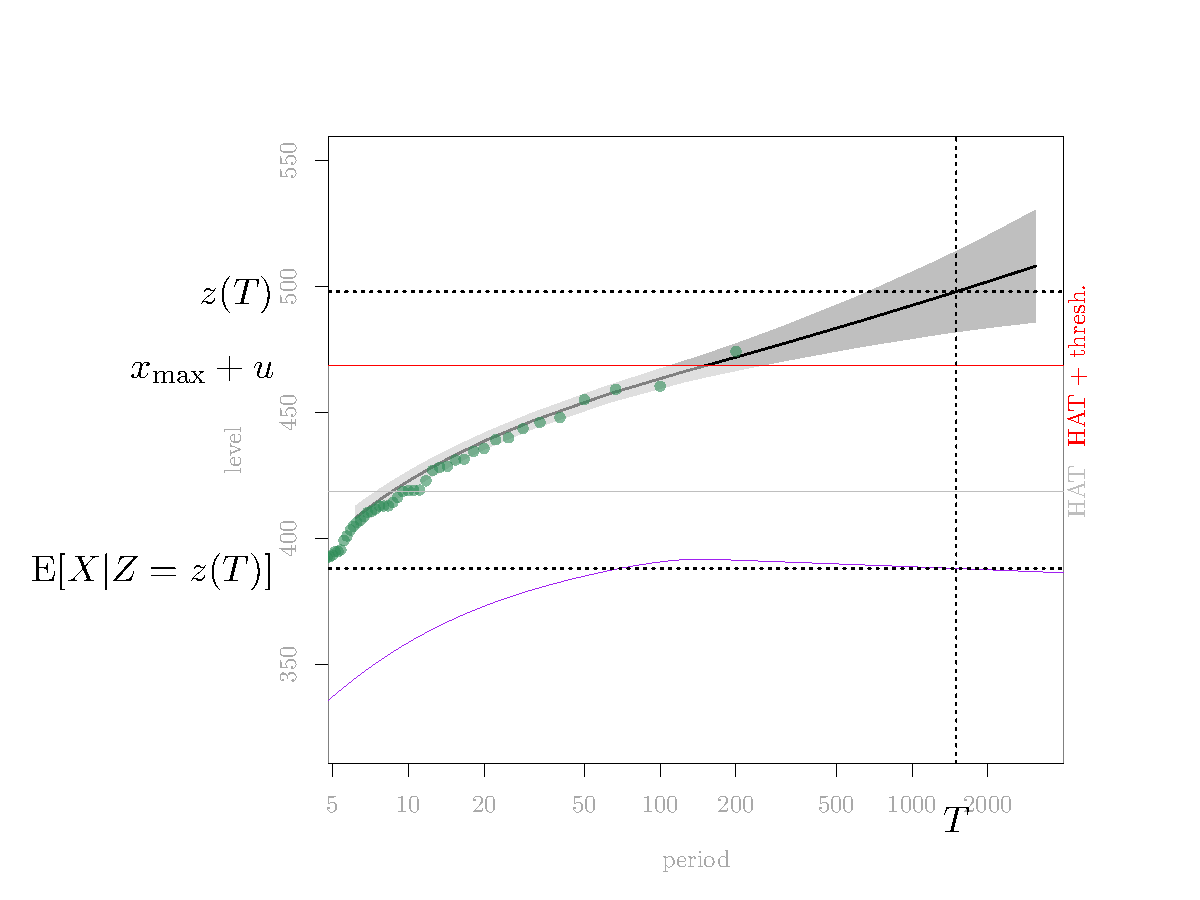
\includegraphics[width=12cm]{figures/figure/RLplot-1.pdf} 
   \end{tabular}
   \caption{\label{FigReturnLevel} Return level plot.  Empirical
     points can be shown. When a POT surge model with threshold $u$ is
     used, only levels $> \Up{x} + u$ must be considered. }
\end{figure}


The return level plot of \textbf{SeaLev} relies on the \verb@RSLplot@
function, which is called e.g. by \verb@convSL@. It shows a distribution as
a curve with points $[T,\,z(T)]$ where $z(T)$ is obtained
by~(\ref{eq:RETLEV2}). A logarithmic scale is used for periods, and an
ordinary scale for levels, thus the points actually plotted are
couples $[\log(T),\,z(T)]$ where $T = [\lambda \times(1-p)]^{-1}$ and
$z(T)= q_Z(p)$. When the distribution of $Z$ is close to the
exponential, the theoretical curve is nearly a straight line. This
will also be true for large return periods if the distribution of $Z$
falls in the Gumbel domain of attraction.

In the present context, the interest is focused on the sea level~$Z$.
Since the distribution of $Z$ results from the convolution and not from an
estimation, there will generally be no use of experimental
values for $Z$. In the POT context, the computation is exact only
for $z > \Up{x} + u$, and thus \textit{only the corresponding part of the
return level curve must be used then}.

A curve showing the value of the conditional expectation $\Esp\bCond{X}{Z}$
for $Z = z(T)$ is shown. In some cases, this curve may not be seen because
of the limits of the axes. It is possible to change these limits, see
section~\ref{AdjustRLplot} later.

Experimental extreme values of the sea level can be displayed on the return
level plot by using suitable plotting positions.  
\index{experimental points}\index{plotting positions}\index{r largest@{$r$ largest}}
Assume that we are given the $r$ largest values $Z_k$ of the sea level during a
period with known duration $w$. The underlying total number of seal levels
$n_{\texttt{H}}$ is the number of high tides corresponding to the yearly rate
$\lambda_{\texttt{H}} =705.8\,{\textrm{year}}^{-1}$. Assuming that the $Z_k$ are
in decreasing order, the return period $\widetilde{T}_k$ used for $Z_k$ is such
that $1/(\lambda_{\texttt{H}}\,\widetilde{T}_k)$ is the estimated probability of
exceedance of $Z_k$, i.e.
$$
    \frac{1}{\lambda_{\texttt{H}}\,\widetilde{T}_k} = \frac{k}{n_{\texttt{H}}+1} = 
    \frac{k}{\lambda_{\texttt{H}} w +1}, 
$$
where the duration~$w$ is assumed to be in years. For instance if $w=10\,\textrm{years}$,
the largest experimental level $Z_1$ is considered as the largest 
value among $n_{\texttt{H}}=705.8 \times 10 = 7058$ levels, corresponding
to a probability of exceedance of $1/7059$, and to a return period 
of $7059/705.8 \approx 10$~years.
The rationale of the formula is
that the tides $X_k$ corresponding to the $Z_k$ are assumed to occur
at the same rate as randomly chosen tides. See section~\ref{EMPPOINTS} 
page~\pageref{EMPPOINTS} for an example.


\section{Special case: GPD surges }
%%------------------------------------------------------

\subsection{Exponential surges}
%%-----------------------------------
\label{ExpSurges} 
\index{exponential distribution|(}
A special case of interest is when $Y$ has an exponential distribution with
location $\mu_Y$ and scale $\sigma_Y$.
It turns out then that the distribution of $Z$ conditional on $Z > \Up{x} + \mu_Y$ 
is also exponential. More precisely for $z > \Up{x} + \mu_Y$ the value
of the survival $S_Z(z)$ is identical to $S_{Z^\star}(z)$ with $Z^\star := \mu_X^\star + Y$ and
\begin{equation}
  \label{eq:muXStar}
  \mu_X^\star := \sigma_Y \log \Esp\left[ e^{X / \sigma_Y} \right] = \sigma_Y K_X(1 / \sigma_Y),
\end{equation}
where $K_X(t) := \log \Esp[e^{tX}]$ is the generating function of the
cumulants of~$X$. In other words, except for small return periods, the
return levels of $Z$ are identical to those that would be obtained
with a constant astronomical tide $X \equiv \mu_X^\star$. We also have
then
$$
\Esp\bCond{X}{Z=z} = \mu_X^\star \qquad \text{for }z > \Up{x} + \mu_Y.
$$ 
Note that $\Esp[X] \leqslant \mu_X^\star \leqslant \Up{x}$, so the
expected tide corresponding to large sea levels~$Z$ falls somewhere
between the unconditional mean tide and the maximal tide.
\index{cumulants (generating function of)}
\index{exponential distribution|)}

\subsection{GPD surges}
%%-------------------------
\index{GPD (Generalised Pareto Distribution)|(} When the surge $Y$ has
a GP distribution $\texttt{GPD}(\mu_Y,\,\sigma_Y,\,\xi_Y)$, the
distribution of $Z$ is a continuous mixture of GPDs with scale
$\sigma_Y$ and scale $\xi_Y$. The tail of $Z$ will resemble that of
$Y$, with three possible behaviours.

\begin{itemize}

\item When $\xi_Y<0$ the distribution of $Z$ has a finite upper end-point
  $\Up{z} = \Up{x} + \Up{y} < \infty$. The conditional expectation 
  $\Esp\bCond{X}{Z=z}$ tends to $\Up{x}$ for $z \to \infty$.

\item When $\xi_Y = 0$, the tail distribution of $Z$ is exponential
  with scale $\sigma_Y$. The conditional expectation
  $\Esp\bCond{X}{Z=z}$ is equal to $\mu_X^\star$ in (\ref{eq:muXStar})
  for $z > \Up{x} + \mu_Y$.

\item When $\xi_Y>0$ it can be shown that $Z$ is
  \textit{tail-equivalent} to $Y$, i.e.  $S_Z(z) / S_Y(z)$ tends to
  $1$ when $z \to \infty$. So $Y$ is heavy-tailed. The conditional
  expectation $\Esp\bCond{X}{Z=z}$ tends to $\Esp[X]$ for $z \to
  \infty$.
  
  \index{tail-equivalent}
  
\end{itemize}

When the shape is small $\xi_Y \approx 0$, the distribution of $Z$ can
be approximated as $\texttt{GPD}(\mu_X^\star +
\mu_Y,\,\sigma_Y,\,\xi_Y)$ with $\mu_X^\star$ as above
in~(\ref{eq:muXStar}).

\begin{remark}
  A comparable approximation is used in~\cite{ColesCoastalFlood} for
  annual maxima of sea level modelled with a GEV distribution. The
  impact of the tide on the distribution of annual maximal sea levels
  is simply to shift the distribution of annual maximal surges. The
  value of the shift is the average value of $\sigma
  \exp(X_t/\sigma)$, where $\sigma$ is the GEV scale parameter which
  plays the same role as the GPD scale for the tail distribution. In
  view of (\ref{eq:ERGOS}) above for the function $\phi := \exp$, the
  shift is a close approximation to~$\mu_X^\star$.
  
  \index{GEV (Generalised Extreme Value)}

\end{remark}

\index{GPD (Generalised Pareto Distribution)|)}


\chapter{Using the \code{convSL} function}
%%==============================================
\section{Goals}
%%--------------------------------------
The \verb@convSL@ function computes return levels for the sea level
$Z$ using the distributions for $X$ and $Y$ given on input.  It
returns a list with several objects, among which a ``prediction'' table
associating return periods or probabilities to return levels. When
possible, approximate confidence limits are computed using the delta
method.

This function is not concerned with estimation tasks (e.g. POT), which should
rely on other packages.


\section{Non-parametric density of $X$}
%%--------------------------------------
The density of $X$ can be provided as a list with elements \code{x}
and \code{y}. It can be an R object of the (S3) class \verb@density@,
such as computed with the \verb@density@ function of the \pkg{stats}
package. The range of $X$ is obtained as the range of the \verb@x@
element of the list.

The dataset \verb@Brest.tide@ from \verb@SeaLev@ provides
an example of estimated density for high-tide sea levels in Brest.
The \verb@plot@ function call and subsequent graphics calls produce the
plot on the left of the figure~\ref{BrestTide}.

\begin{knitrout}
\definecolor{shadecolor}{rgb}{0.969, 0.969, 0.969}\color{fgcolor}\begin{kframe}
\begin{alltt}
\hlkwd{library}\hlstd{(SeaLev)}
\hlkwd{data}\hlstd{(Brest.tide)}
\hlkwd{class}\hlstd{(Brest.tide)}
\end{alltt}
\begin{verbatim}
## [1] "list"
\end{verbatim}
\begin{alltt}
\hlkwd{str}\hlstd{(Brest.tide)}
\end{alltt}
\begin{verbatim}
## List of 2
##  $ x: num [1:512] 100 101 102 102 103 ...
##  $ y: num [1:512] 0.00 5.84e-06 1.12e-05 1.66e-05 2.20e-05 ...
\end{verbatim}
\begin{alltt}
\hlkwd{plot}\hlstd{(Brest.tide,} \hlkwc{col} \hlstd{=} \hlstr{"SeaGreen"}\hlstd{,} \hlkwc{type} \hlstd{=} \hlstr{"l"}\hlstd{,}
     \hlkwc{main} \hlstd{=} \hlstr{"Density of high-tide sea level in Brest"}\hlstd{)}
\hlkwd{grid}\hlstd{();} \hlkwd{abline}\hlstd{(}\hlkwc{h} \hlstd{=} \hlnum{0}\hlstd{)}
\end{alltt}
\end{kframe}
\end{knitrout}

\noindent
The level $X$ is given here in centimetres, the density values are
accordingly in $\textrm{cm}^{-1}$.  As implicitly admitted when
plotting densities, it will be assumed that linear interpolation can
be used to evaluate $f_X(x)$ on another grid of values, usually a
finer one. The required normalisation condition is that the
trapezoidal rule for numerical integration should lead to an integral
equal to~$1.0$. Provided that the density values are zero at
end-points, the rectangles rule should also give the same value~$1.0$.

\begin{knitrout}
\definecolor{shadecolor}{rgb}{0.969, 0.969, 0.969}\color{fgcolor}\begin{kframe}
\begin{alltt}
\hlstd{Brest.tide}\hlopt{$}\hlstd{y[}\hlkwd{c}\hlstd{(}\hlnum{1L}\hlstd{,} \hlkwd{length}\hlstd{(Brest.tide}\hlopt{$}\hlstd{y))]}
\end{alltt}
\begin{verbatim}
## [1] 0 0
\end{verbatim}
\begin{alltt}
\hlstd{h} \hlkwb{<-} \hlkwd{diff}\hlstd{(Brest.tide}\hlopt{$}\hlstd{x)[}\hlnum{1}\hlstd{]}
\hlstd{h} \hlopt{*} \hlkwd{sum}\hlstd{(Brest.tide}\hlopt{$}\hlstd{y)}
\end{alltt}
\begin{verbatim}
## [1] 1
\end{verbatim}
\end{kframe}
\end{knitrout}

\noindent
These checks could be replaced in future versions by the registration
of a formal class for discredited densities.

\section{Convolution}
%%======================
\subsection{Specifying parameters for $Y$}
%----------------------------
The parameter values (generally estimated) must be given as a named
list or a numeric vector with named elements. For instance, consider 
the high-tide skew surges for Brest, and assume that in a POT analysis using
a threshold $u=50$ cm we got the estimated parameters $\sigma_Y = 10$~cm
(scale) $\xi_Y = -0.01$ (shape), and that the exceedances occurred
at a rate of \verb@1.6@~$\mathrm{years}^{-1}$. 
\index{rate, sampling for high tides}
\index{skew surge}
We can store these informations
as R objects say \verb@u@, \verb@theta.y@ and \verb@lambda@

\begin{knitrout}
\definecolor{shadecolor}{rgb}{0.969, 0.969, 0.969}\color{fgcolor}\begin{kframe}
\begin{alltt}
\hlstd{u} \hlkwb{<-} \hlnum{50}
\hlstd{theta.y} \hlkwb{<-} \hlkwd{c}\hlstd{(}\hlstr{"scale"} \hlstd{=} \hlnum{10}\hlstd{,} \hlstr{"shape"} \hlstd{=} \hlopt{-}\hlnum{0.01}\hlstd{)}
\hlstd{lambda} \hlkwb{<-} \hlnum{1.6}
\end{alltt}
\end{kframe}
\end{knitrout}

\noindent
Note that we can use a named numeric vector created with the \verb@c@
function or a \verb@list@, but in both cases the element names must
match the parameters names of the distribution.  Now we can use the
created objects as values for the formal arguments \verb@threshold.y@,
 \verb@par.y@ and \verb@lambda@ of the convolution function.

\begin{knitrout}
\definecolor{shadecolor}{rgb}{0.969, 0.969, 0.969}\color{fgcolor}\begin{kframe}
\begin{alltt}
\hlstd{conv.gpd0} \hlkwb{<-} \hlkwd{convSL}\hlstd{(}\hlkwc{dens.x} \hlstd{= Brest.tide,}
                   \hlkwc{threshold.y} \hlstd{= u,} \hlkwc{distname.y} \hlstd{=} \hlstr{"GPD"}\hlstd{,}
                   \hlkwc{lambda} \hlstd{= lambda,} \hlkwc{par.y} \hlstd{= theta.y,}
                   \hlkwc{main} \hlstd{=} \hlstr{"Sea-level with GPD surges: given parameters"}\hlstd{)}
\end{alltt}
\end{kframe}
\end{knitrout}

\index{return level plot}
\noindent
By default, a return level plot is produced as in figure~\ref{BrestTide}. No ``confidence
band'' can be plotted here since no information was given about 
estimation uncertainty. 

\begin{figure}
   \centering
   \begin{tabular}{c c} 
     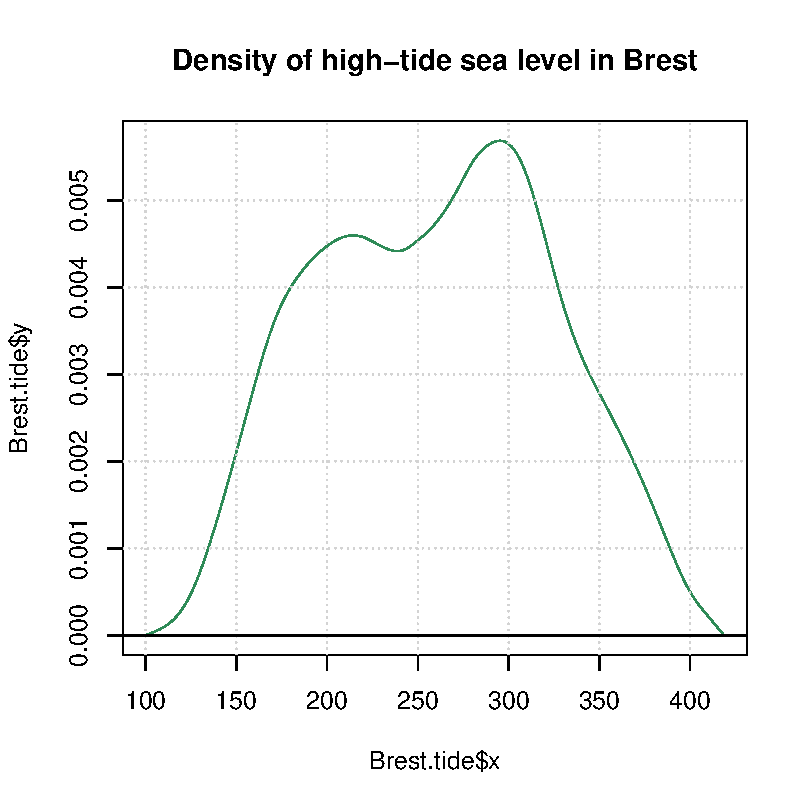
\includegraphics[width=7.4cm]{Rgraphics/figBrestTide-1.pdf} &
     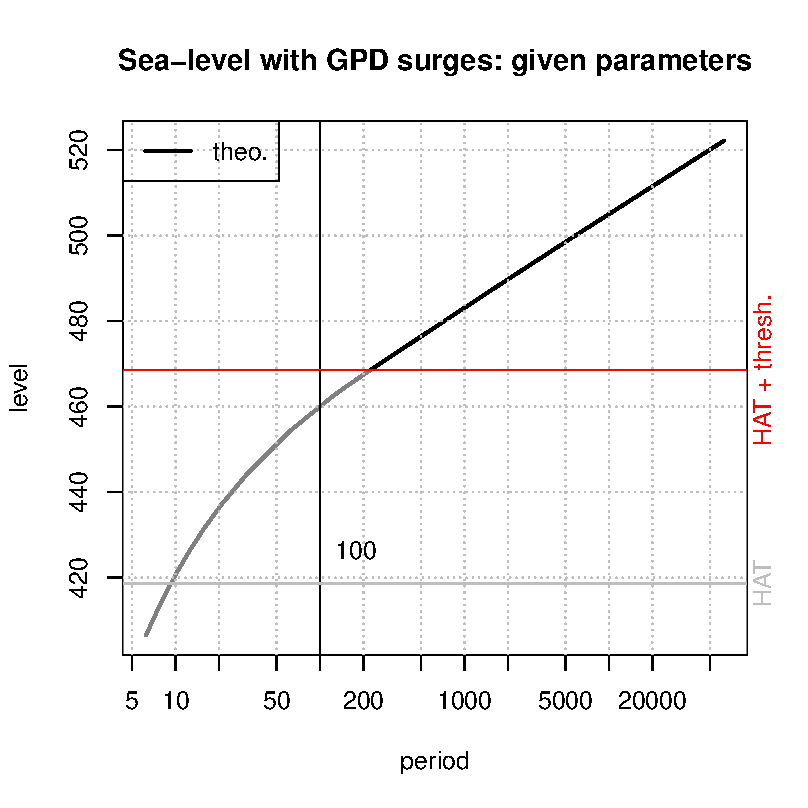
\includegraphics[width=7.4cm]{Rgraphics/figBrestConv0-1.pdf} 
     %%\includegraphics[width=7.4cm]{Rgraphics/figRenplotGaronne.pdf} 
   \end{tabular}
   \caption{\label{BrestTide}Left panel:  density of the high-tide 
   sea level $X$ in Brest (France). Right panel: return level plot 
   using convolution and a known GPD distribution for the surge $Y$. 
   Only the part above the horizontal red line should be used, 
   corresponding to return periods over about $200$~years. 
 }
\end{figure}

\subsection{Using a fitted POT model}
%%---------------------------------
\index{POT (Peak Over the Threshold)}
The estimated values for the surge can be computed using
\textbf{Renext} and its \verb@Brest@ dataset.  The arguments to be
passed to the \verb@Renouv@ function then include the vector of surges
\verb@x@ and the effective duration (in years) in order to estimate
the rate \verb@lambda@ (in inverse years).


\begin{knitrout}
\definecolor{shadecolor}{rgb}{0.969, 0.969, 0.969}\color{fgcolor}\begin{kframe}
\begin{alltt}
\hlkwd{library}\hlstd{(Renext);} \hlkwd{data}\hlstd{(Brest)}
\hlstd{fit.gpd1} \hlkwb{<-} \hlkwd{Renouv}\hlstd{(}\hlkwc{x} \hlstd{= Brest}\hlopt{$}\hlstd{OTdata}\hlopt{$}\hlstd{Surge,}
                   \hlkwc{effDuration} \hlstd{=} \hlkwd{as.numeric}\hlstd{(Brest}\hlopt{$}\hlstd{OTinfo}\hlopt{$}\hlstd{effDuration),}
                   \hlkwc{threshold} \hlstd{=} \hlnum{50}\hlstd{,} \hlkwc{distname.y} \hlstd{=} \hlstr{"GPD"}\hlstd{,}
                   \hlkwc{main} \hlstd{=} \hlstr{"GPD surge"}\hlstd{)}
\hlkwd{coef}\hlstd{(fit.gpd1)}
\end{alltt}
\begin{verbatim}
##       lambda        scale        shape 
##  1.612247663 10.667124374 -0.006425839
\end{verbatim}
\end{kframe}
\end{knitrout}


The estimated parameters are very close to those used before.  The fit
produces the return level plot shown on the left of~\ref{BrestSurge}, with a
$100$-years return level of about $100$~cm. The fitted object contains a
covariance matrix of estimation.
\begin{knitrout}
\definecolor{shadecolor}{rgb}{0.969, 0.969, 0.969}\color{fgcolor}\begin{kframe}
\begin{alltt}
\hlstd{cov1} \hlkwb{<-} \hlkwd{vcov}\hlstd{(fit.gpd1)}
\hlstd{cov1}
\end{alltt}
\begin{verbatim}
##            lambda       scale        shape
## lambda 0.01092161  0.00000000  0.000000000
## scale  0.00000000  0.95005346 -0.044531845
## shape  0.00000000 -0.04453185  0.004147856
\end{verbatim}
\end{kframe}
\end{knitrout}
\noindent
This matrix can be used in the \verb@covpar.y@ formal argument of
\verb@convSL@ function. As it is the case here, the matrix must have
rownames and colnames, and these must agree with the parameter names
of the distribution.


\noindent
We get the return level at the right of figure~\ref{BrestSurge}, in
which (pointwise) confidence bands are drawn for the return levels.
These are obtained by ``propagating the uncertainty'' on the parameters (as
quantified by the covariance) to the return levels~$z(T)$. This is
done using the delta method and the partial
derivatives~(\ref{eq:DERT}).
\index{delta method}

The plot can be enhanced by filling the confidence region(s) and
using colours. The confidence levels can be set using \verb@pct.conf@.
\index{confidence bands!filled}
\index{confidence bands!percentage}

\begin{knitrout}
\definecolor{shadecolor}{rgb}{0.969, 0.969, 0.969}\color{fgcolor}\begin{kframe}
\begin{alltt}
\hlstd{conv.gpd2a} \hlkwb{<-} \hlkwd{convSL}\hlstd{(}\hlkwc{dens.x} \hlstd{= Brest.tide,}
                     \hlkwc{threshold.y} \hlstd{=} \hlnum{50}\hlstd{,}
                     \hlkwc{distname.y} \hlstd{=} \hlstr{"GPD"}\hlstd{,}
                     \hlkwc{lambda} \hlstd{= lambda,} \hlkwc{par.y} \hlstd{= theta.y,}
                     \hlkwc{pct.conf} \hlstd{=} \hlkwd{c}\hlstd{(}\hlnum{95}\hlstd{,} \hlnum{90}\hlstd{),}
                     \hlkwc{filled.conf} \hlstd{=} \hlnum{TRUE}\hlstd{,} \hlkwc{mono} \hlstd{=} \hlnum{FALSE}\hlstd{,}
                     \hlkwc{covpar.y} \hlstd{= cov1,}
                     \hlkwc{main} \hlstd{=} \hlstr{"Sea-level for Brest with GPD surges (lambda known)"}\hlstd{)}
\end{alltt}
\end{kframe}
\end{knitrout}

\noindent
The plot is shown on the left panel of figure~\ref{BrestSurge2}.

It is possible to use in \verb@convSL@ a covariance matrix without the
elements related to the rate \verb@"lambda"@. For instance, dropping
the first row and the first column in \verb@cov1@

\begin{knitrout}
\definecolor{shadecolor}{rgb}{0.969, 0.969, 0.969}\color{fgcolor}\begin{kframe}
\begin{alltt}
\hlstd{cov1[}\hlopt{-}\hlnum{1}\hlstd{,} \hlopt{-}\hlnum{1}\hlstd{]}
\end{alltt}
\begin{verbatim}
##             scale        shape
## scale  0.95005346 -0.044531845
## shape -0.04453185  0.004147856
\end{verbatim}
\end{kframe}
\end{knitrout}

\noindent
leads to a matrix that can be used with \verb@convSL@. The same
effect can be obtained by specifying a \verb@use.covlambda@ argument
with \verb@FALSE@ as its value. 
\begin{knitrout}
\definecolor{shadecolor}{rgb}{0.969, 0.969, 0.969}\color{fgcolor}\begin{kframe}
\begin{alltt}
\hlstd{conv.gpd2} \hlkwb{<-} \hlkwd{convSL}\hlstd{(}\hlkwc{dens.x} \hlstd{= Brest.tide,}
                    \hlkwc{threshold.y} \hlstd{=} \hlnum{50}\hlstd{,}
                    \hlkwc{distname.y} \hlstd{=} \hlstr{"GPD"}\hlstd{,}
                    \hlkwc{lambda} \hlstd{= lambda,} \hlkwc{par.y} \hlstd{= theta.y,}
                    \hlkwc{use.covlambda} \hlstd{=} \hlnum{FALSE}\hlstd{,}
                    \hlkwc{pct.conf} \hlstd{=} \hlkwd{c}\hlstd{(}\hlnum{95}\hlstd{,} \hlnum{90}\hlstd{),}
                    \hlkwc{filled.conf} \hlstd{=} \hlnum{TRUE}\hlstd{,} \hlkwc{mono} \hlstd{=} \hlnum{FALSE}\hlstd{,}
                    \hlkwc{covpar.y} \hlstd{= cov1,}
                    \hlkwc{main} \hlstd{=} \hlstr{"Sea-level for Brest with GPD surges (lambda known)"}\hlstd{)}
\end{alltt}
\end{kframe}
\end{knitrout}
\noindent
The plot is shown on the right panel of
figure~\ref{BrestSurge2}. The effect of ignoring the uncertainty on
\verb@lambda@ is to produce a narrower confidence band for small
return periods. The effect for large periods is negligible.

\begin{figure}
   \centering
   \begin{tabular}{c c} 
     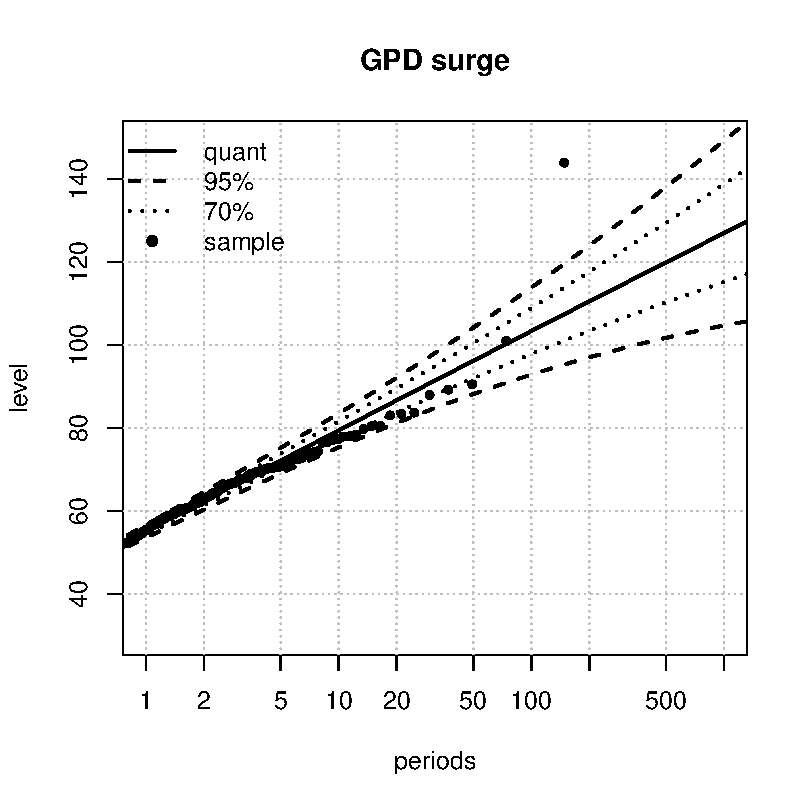
\includegraphics[width=7.4cm]{Rgraphics/figBrestFitSurge-1.pdf} &
     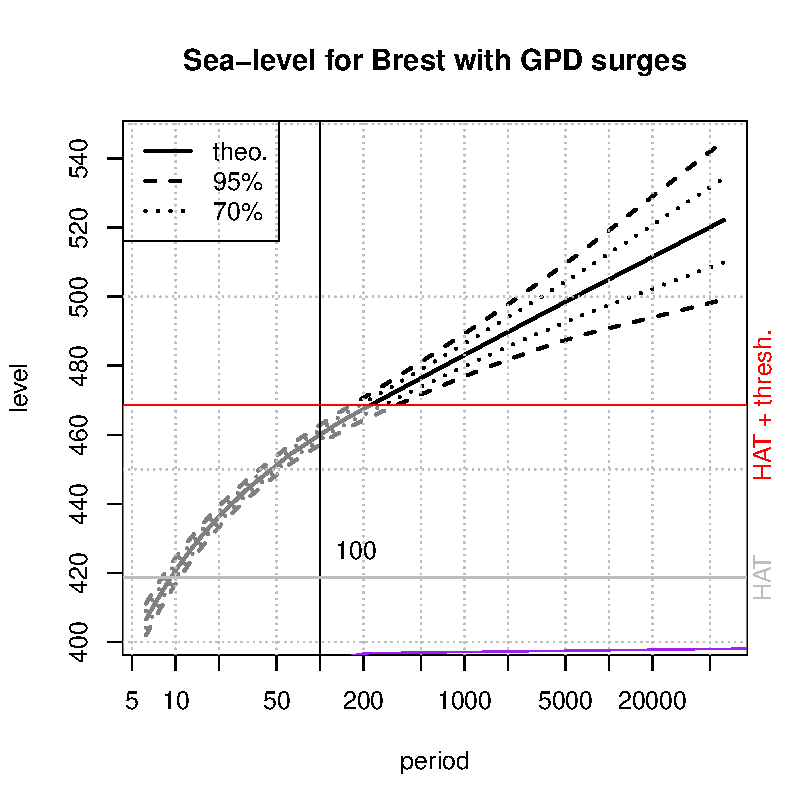
\includegraphics[width=7.4cm]{Rgraphics/figBrestConv1-1.pdf}  
   \end{tabular}
   \caption{\label{BrestSurge} Fitting a POT model for Brest surge with \textbf{Renext} (left),
     and using the fitted distribution within a convolution.
   }
\end{figure}

\begin{figure}
   \centering
   \begin{tabular}{c c} 
     %%\includegraphics[width=7.4cm]{Rgraphics/figBrestFitSurge.pdf} &
     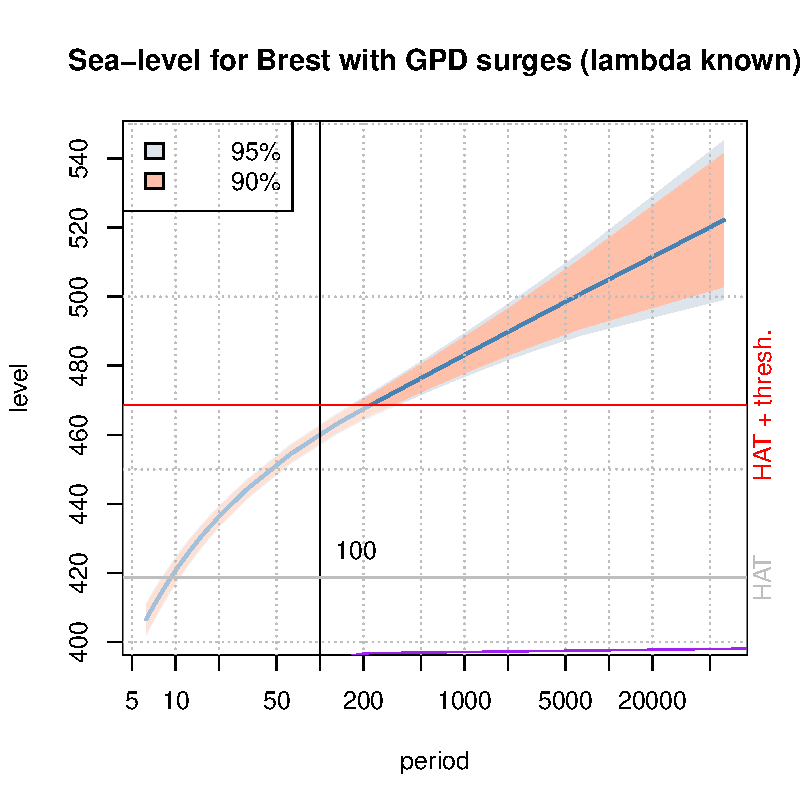
\includegraphics[width=7.4cm]{Rgraphics/figBrestConv15-1.pdf} 
     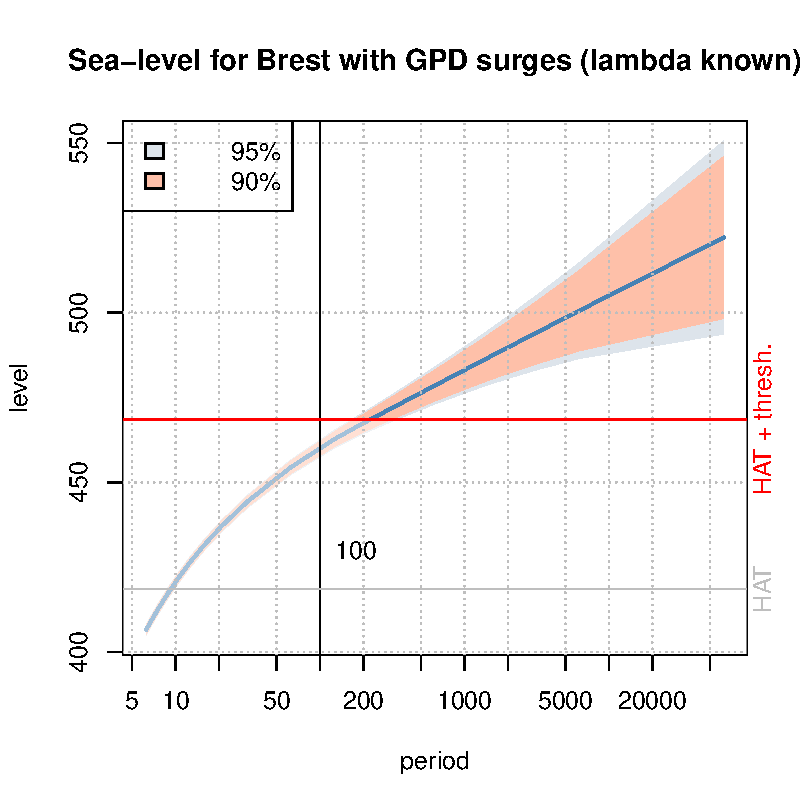
\includegraphics[width=7.4cm]{Rgraphics/figBrestConv2-1.pdf}  
   \end{tabular}
   \caption{\label{BrestSurge2} Comparison of two convolutions of the
     tide with the fitted GPD.  On the left panel, the covariance
     concerns \texttt{lambda}. Right panel \texttt{use.covlambda =
       FALSE}. }
\end{figure}

\subsection{Using a fitted non-POT model}
%%---------------------------------
\label{NONPOT}
Although a POT model will be used in most cases, it is yet possible to
use a non-POT model, i.e.  a non-conditional distribution for~$Y$.
For illustration purpose only, assume that the surge at Brest can be
described by a Gumbel \index{Gumbel distribution} distribution with
parameters $\mu_Y=-10.8$~cm (location) and $\sigma_Y= 10$~cm (scale).  The
Gumbel assumption for surges is very close to that of exponentially
distributed excesses over a high enough threshold. Here the
parameters were chosen in accordance with the POT estimation: $\sigma_Y$
takes the same values as in the GPD case, while $\mu_Y$ was chosen to
give the same rate of exceedance over $u = 50$~\textrm{cm}.  
\index{GEV (Generalised Extreme Value)}

The arguments provided to \verb@convSL@ will be quite different than
in the GPD case.  We specify a non-POT distribution by using a
\verb@threshold.y@ with value \verb@NA@, and the rate \verb@lambda@
must now be $705.8\,\textrm{years}^{-1}$.

\begin{knitrout}
\definecolor{shadecolor}{rgb}{0.969, 0.969, 0.969}\color{fgcolor}\begin{kframe}
\begin{alltt}
\hlstd{par.y} \hlkwb{<-} \hlkwd{c}\hlstd{(}\hlkwc{loc} \hlstd{=} \hlopt{-}\hlnum{10.8}\hlstd{,} \hlkwc{scale} \hlstd{=} \hlnum{10}\hlstd{)}
\hlstd{res.gumbel} \hlkwb{<-} \hlkwd{convSL}\hlstd{(}\hlkwc{dens.x} \hlstd{= Brest.tide,}
                     \hlkwc{threshold.y} \hlstd{=} \hlnum{NA}\hlstd{,}
                     \hlkwc{distname.y} \hlstd{=} \hlstr{"gumbel"}\hlstd{,}
                     \hlkwc{lambda} \hlstd{=} \hlnum{705.8}\hlstd{,}
                     \hlkwc{par.y} \hlstd{= par.y,}
                     \hlkwc{filled.conf} \hlstd{=} \hlnum{TRUE}\hlstd{,} \hlkwc{mono} \hlstd{=} \hlnum{FALSE}\hlstd{,}
                     \hlkwc{main} \hlstd{=} \hlstr{"Gumbel surges"}\hlstd{)}
\end{alltt}
\end{kframe}
\end{knitrout}

\noindent
The return level is shown on figure~\ref{BrestSurgeGEV}.  Note that
\verb@threshold.y@ is equal to its default value \verb@NA@ and that we
could have left \verb@lambda@ to its default value since this is
$705.8$ when \verb@lambda@ is \verb@NA@ (see the package manual). Thus
these two arguments could have been omitted in the call.

\begin{figure}
   \centering
   \begin{tabular}{c c} 
     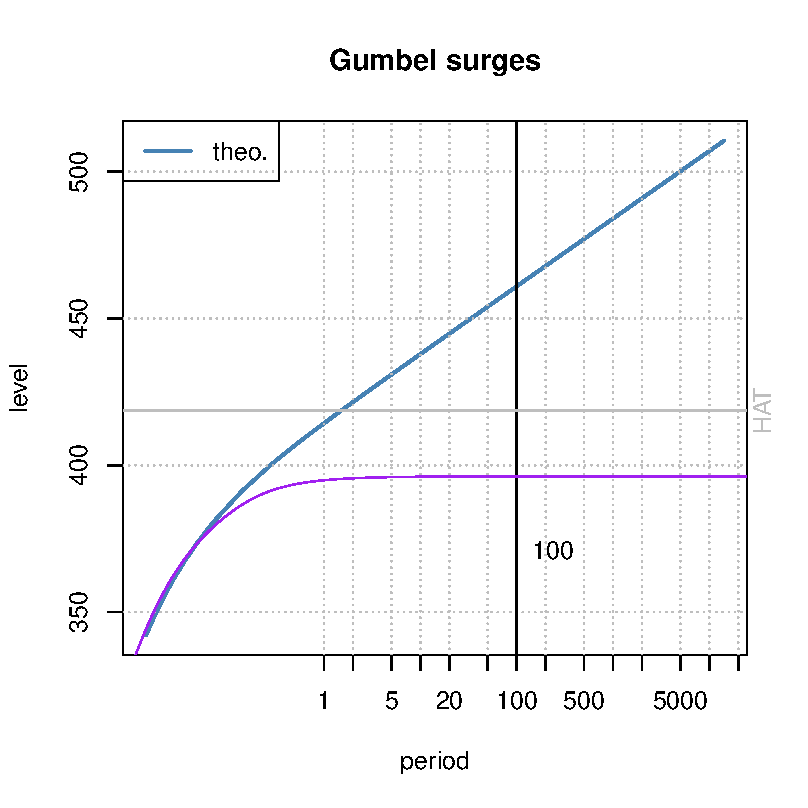
\includegraphics[width=7.4cm]{Rgraphics/figBrestConvGEV-1.pdf} 
     %%\includegraphics[width=7.4cm]{Rgraphics/figBrestConv2.pdf}  
   \end{tabular}
   \caption{\label{BrestSurgeGEV} Using a Gumbel distribution
     (non-POT) for the surge. Note that the horizontal line $\Up{x} +
     u$ shown for POT surges no longer exists.}
\end{figure}

\begin{remark}
  By using \verb@lambda = 705.8@ we assume that the given distribution
  for~$Y$ is for an arbitrary skew surge as
  in~\cite[chap.~VIII]{SIMON}. If instead we aim to use the
  a\textit{nnual maximal surge}, then we must use \verb@lambda = 1.0@
  with a suitable distribution.
  %% Due to the max-stability of the Gumbel distribution we
  %% will obtain the same return level curve if we replace $\lambda$ by 
  %% $\widetilde{\lambda} := \lambda/n$ and $\mu_Y$ by $\widetilde{\mu}_Y := \mu_Y + \sigma_Y \log n$
  %% for any positive $n$.
\end{remark}


\section{Predictions}
%%---------------------
The computed return levels and confidence limits are returned within a
data.frame \verb@pred@. Here are the first rows.

\begin{knitrout}
\definecolor{shadecolor}{rgb}{0.969, 0.969, 0.969}\color{fgcolor}\begin{kframe}
\begin{alltt}
\hlkwd{head}\hlstd{(conv.gpd2}\hlopt{$}\hlstd{pred,} \hlkwc{n} \hlstd{=} \hlnum{3}\hlstd{)}
\end{alltt}
\begin{verbatim}
##         prob period    quant     L.95     U.95     L.90     U.90
## 100 0.993750    100 460.1913 457.7357 462.6469 458.1305 462.2521
## 200 0.996875    200 467.4752 464.3794 470.5711 464.8771 470.0733
## 500 0.998750    500 476.4099 471.5000 481.3198 472.2894 480.5304
\end{verbatim}
\end{kframe}
\end{knitrout}

\noindent
Each row correspond to a given period $T$, e.g. $T=100$ years, and
give the corresponding probability of non-exceedance $p(T)$ (column
\verb@prob@), the corresponding return level $z(T)$ (column
\verb@quant@) as well as confidence limits for $z(T)$, here $70$~pct
and $95$~pct.  It is possible to specify the wanted periods by using
the \verb@pred.period@ formal of \verb@Renouv@.


Recall that $z(T)$ and $p(T)$ are connected to each other by $z =
1/[\widehat{\lambda} \times (1-p)]$, thus the relation between $T$ and
$p$ is affected by the uncertainty on the estimation of
$\lambda$. However, this uncertainty is small for large periods.

\index{prediction}
Also note that the term ``prediction'' can be misleading. The $100$-years
return level is the level that is exceeded on average once every
$100$~years. This level might occur twice or more in a given century.

When a POT model is used for the surges~$Y$, only periods corresponding
to levels $z > \Up{x} + u$ must be used, where $u$ is the threshold.

\section{Adjusting the return level plot}
%%-------------------------------------
\label{AdjustRLplot}
\index{axes, controlling the range}
The axis limits can be adjusted using the \verb@ylim@ parameters and
the ``dots'' mechanism just like as for the \verb@main@ formal.  It
will generally be necessary to modify \verb@ylim@ in order to see the
conditional expectation curve~$\Esp\pCond{X}{Z=z}$ as in

\begin{knitrout}
\definecolor{shadecolor}{rgb}{0.969, 0.969, 0.969}\color{fgcolor}\begin{kframe}
\begin{alltt}
\hlstd{conv.gpd3} \hlkwb{<-} \hlkwd{convSL}\hlstd{(}\hlkwc{dens.x} \hlstd{= Brest.tide,}
                    \hlkwc{threshold.y} \hlstd{=} \hlnum{50}\hlstd{,} \hlkwc{distname.y} \hlstd{=} \hlstr{"GPD"}\hlstd{,}
                    \hlkwc{lambda} \hlstd{= lambda,} \hlkwc{par.y} \hlstd{= theta.y,} \hlkwc{covpar.y} \hlstd{= cov1,}
                    \hlkwc{ylim} \hlstd{=} \hlkwd{c}\hlstd{(}\hlnum{300}\hlstd{,} \hlnum{600}\hlstd{),}
                    \hlkwc{main} \hlstd{=} \hlstr{"Sea-level for Brest with GPD surges (lambda known)"}\hlstd{)}
\end{alltt}
\end{kframe}
\end{knitrout}

\noindent
leading to the plot on left of figure~\ref{BrestSurge3}. 

For the x-axis, which is in log-scale, it is preferable to work
\verb@Tlim@ which allows to give the two limits in years.

\begin{knitrout}
\definecolor{shadecolor}{rgb}{0.969, 0.969, 0.969}\color{fgcolor}\begin{kframe}
\begin{alltt}
\hlstd{conv.gpd3} \hlkwb{<-} \hlkwd{convSL}\hlstd{(}\hlkwc{dens.x} \hlstd{= Brest.tide,}
                    \hlkwc{threshold.y} \hlstd{=} \hlnum{50}\hlstd{,} \hlkwc{distname.y} \hlstd{=} \hlstr{"GPD"}\hlstd{,}
                    \hlkwc{lambda} \hlstd{= lambda,} \hlkwc{par.y} \hlstd{= theta.y,} \hlkwc{covpar.y} \hlstd{= cov1,}
                    \hlkwc{Tlim} \hlstd{=} \hlkwd{c}\hlstd{(}\hlnum{100}\hlstd{,} \hlnum{3000}\hlstd{),}
                    \hlkwc{main} \hlstd{=} \hlstr{"Sea-level for Brest with GPD surges (lambda known)"}\hlstd{)}
\end{alltt}
\end{kframe}
\end{knitrout}

\noindent
%% Note that the results are recomputed but the parameters \verb@Tlim@,
%% \verb@problim@ are purely graphical ones and have no impact on the
%% computed results.
The plot can be annotated with the standard functions from the
\textbf{graphics} package: \verb@text@, \verb@lines@, etc.  Since the
$x$-axis is in log-scale it will be simpler to use \verb@par()usr@ to
get the world coordinates or to use the \verb@locator@ function.

\begin{figure}
   \centering
   \begin{tabular}{c c} 
     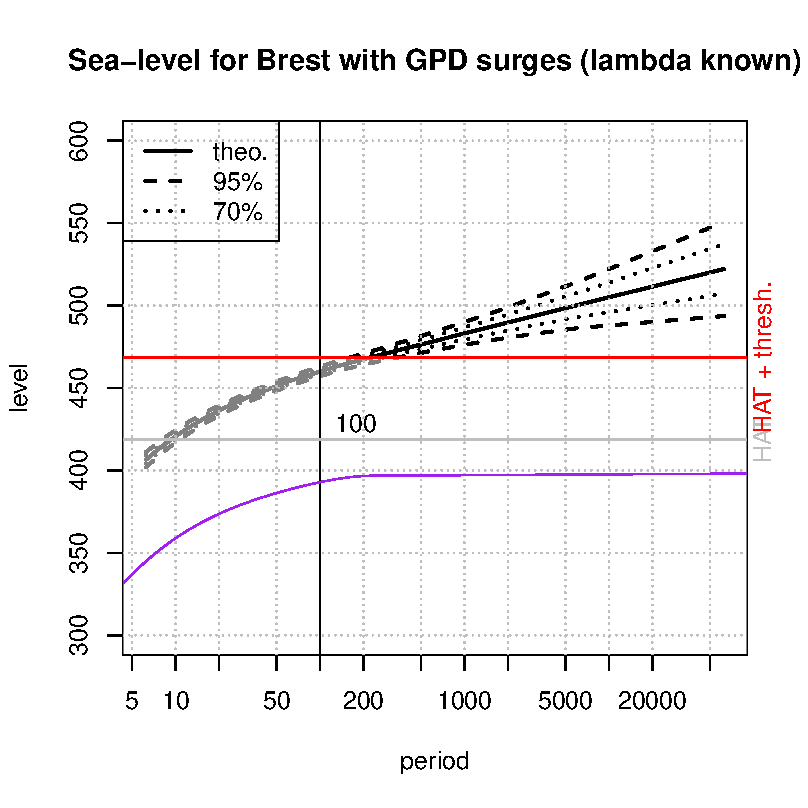
\includegraphics[width=7.4cm]{Rgraphics/figBrestConv3-1.pdf} &
     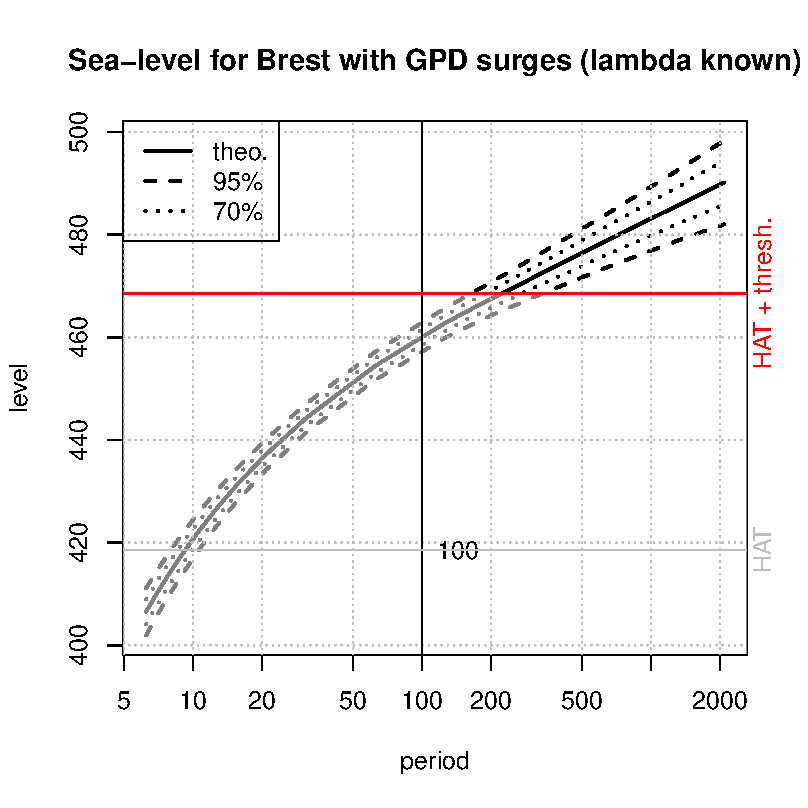
\includegraphics[width=7.4cm]{Rgraphics/figBrestConv4-1.pdf} 
   \end{tabular}
   \caption{\label{BrestSurge3} Changing the axes. Left: the
     \texttt{ylim} argument of \texttt{plot} was used. Right: the
     \texttt{Tlim} argument of \texttt{RSLplot} chooses the range of
     return periods, here from $100$ to $5000$.}
\end{figure}

In order to add experimental points to the plot, the two formal
arguments \index{experimental points}\index{plotting positions}
\verb@z@ and \verb@duration@ must be passed to the \verb@RSLplot@.  In
the simplest case, \verb@z@ is a numeric vector and \verb@duration@ is
a positive numeric value representing a duration in years. 
\label{EMPPOINTS} For instance, with meaningless points and in 
a purely illustrative purpose we get the plots of figure~\ref{empirical}.

\begin{knitrout}
\definecolor{shadecolor}{rgb}{0.969, 0.969, 0.969}\color{fgcolor}\begin{kframe}
\begin{alltt}
\hlstd{res.g2} \hlkwb{<-} \hlkwd{convSL}\hlstd{(}\hlkwc{dens.x} \hlstd{= Brest.tide,}
                 \hlkwc{threshold.y} \hlstd{=} \hlnum{NA}\hlstd{,} \hlkwc{distname.y} \hlstd{=} \hlstr{"gumbel"}\hlstd{,}
                 \hlkwc{lambda} \hlstd{=} \hlnum{705.8}\hlstd{,} \hlkwc{par.y} \hlstd{= par.y,}
                 \hlkwc{filled.conf} \hlstd{=} \hlnum{TRUE}\hlstd{,} \hlkwc{mono} \hlstd{=} \hlnum{FALSE}\hlstd{,}
                 \hlkwc{main} \hlstd{=} \hlstr{"Artificial empirical points (1 set)"}\hlstd{,}
                 \hlkwc{z} \hlstd{=} \hlkwd{c}\hlstd{(}\hlnum{500}\hlstd{,} \hlnum{490}\hlstd{,} \hlnum{480}\hlstd{,} \hlnum{460}\hlstd{),}
                 \hlkwc{duration} \hlstd{=} \hlnum{200}\hlstd{)}
\end{alltt}
\end{kframe}
\end{knitrout}

\noindent
It is possible to specify several vectors using a list for \verb@z@,
the duration being then a vector or a list with the same length as
\verb@z@. 

\begin{knitrout}
\definecolor{shadecolor}{rgb}{0.969, 0.969, 0.969}\color{fgcolor}\begin{kframe}
\begin{alltt}
\hlstd{res.g3} \hlkwb{<-} \hlkwd{convSL}\hlstd{(}\hlkwc{dens.x} \hlstd{= Brest.tide,}
                 \hlkwc{threshold.y} \hlstd{=} \hlnum{NA}\hlstd{,} \hlkwc{distname.y} \hlstd{=} \hlstr{"gumbel"}\hlstd{,}
                 \hlkwc{lambda} \hlstd{=} \hlnum{705.8}\hlstd{,} \hlkwc{par.y} \hlstd{= par.y,}
                 \hlkwc{filled.conf} \hlstd{=} \hlnum{TRUE}\hlstd{,} \hlkwc{mono} \hlstd{=} \hlnum{FALSE}\hlstd{,}
                 \hlkwc{main} \hlstd{=} \hlstr{"Artificial empirical points (2 sets)"}\hlstd{,}
                 \hlkwc{z} \hlstd{=} \hlkwd{list}\hlstd{(}\hlkwd{c}\hlstd{(}\hlnum{500}\hlstd{,} \hlnum{490}\hlstd{,} \hlnum{480}\hlstd{),} \hlkwd{c}\hlstd{(}\hlnum{440}\hlstd{,} \hlnum{420}\hlstd{,} \hlnum{380}\hlstd{,} \hlnum{350}\hlstd{)),}
                 \hlkwc{duration} \hlstd{=} \hlkwd{c}\hlstd{(}\hlnum{200}\hlstd{,} \hlnum{170}\hlstd{))}
\end{alltt}
\end{kframe}
\end{knitrout}

\noindent
Some properties of the points such as the colour can be changed by passing
suitable arguments to the \verb@RLSplot@ function, with names \verb@.points@.
For instance, a vector of colours can be specified with \verb@col.points@.

\begin{figure}
   \centering
   \begin{tabular}{c c} 
     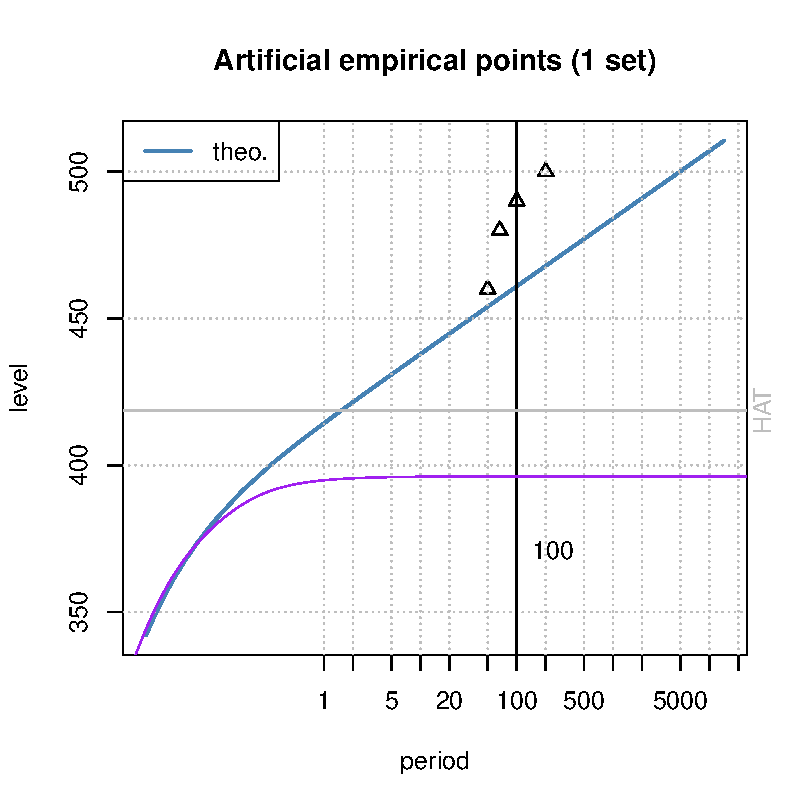
\includegraphics[width=7.4cm]{Rgraphics/figempirical-1.pdf} &
     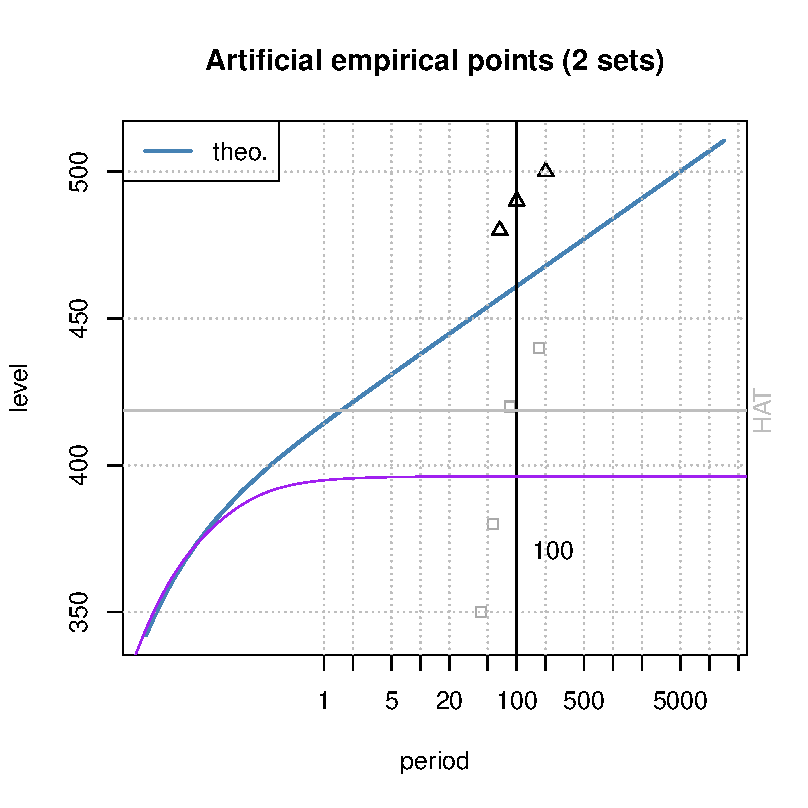
\includegraphics[width=7.4cm]{Rgraphics/figempirical1-1.pdf} 
   \end{tabular}
   \caption{\label{empirical} Adding empirical points to the return level
     plot using \texttt{z} and \texttt{duration}. When several sets are used,
     \texttt{z} must be a list of numeric vectors.}
\end{figure}

\chapter{Spline density for the tide}
%%==============================================

\index{spline density|(}
\index{SplineDensity@{\texttt{SplineDensity}}|see{spline density}}
\index{GPtail@{\texttt{GPtail}}|see{spline density}}

\section{Motivation}
%%-------------------------------
From version \verb@>=0.4-0@ \pkg{SeaLev} allows the use of a spline
density for the tide. Splines can provide a fairly good representation
of general smooth densities with bounded support. Moreover, using a
spline density for $X$ has a special interest here because if $Y \sim
\texttt{GPD}$ the value of the survival $S_Z(z)$ for $z$ large enough
can be given in closed form. Some details are given in
appendix~\ref{AnnSpline}.

\pkg{SeaLev} embeds two main functions dedicated to spline densities.
\begin{itemize}
  
\item \verb@SplineDensity@ creates a spline density with bounded support
  $(\Low{x},\,\Up{x})$. The created object has (S3) class \verb@"SplineDensity"@
  for which a few methods such as \verb@plot@ or \verb@predict@ are provided.
  
  \index{plot method@{\texttt{plot} method}}
  \index{plot method@{\texttt{predict} method}}
  
\item \verb@GPtail@ computes the convolution of a spline density with a 
  GPD. The spline density is provided as an object with class
  \verb@"SplineDensity"@ while the GPD is given by its parameters as 
  in the \code{convSL} function.

\end{itemize}
A few other functions are devoted to the \verb@"SplineDensity"@ class. 

\begin{remark}
  Log-splines are generally preferred to splines for probability densities
  because the positivity constraints are more easily coped with when the
  log-exponential transforms are used. However, the closed form of the
  convolution tail does not exist for a log-spline.
\end{remark}


\section{Example}
%%--------------------
Consider again the astronomical tide at Brest. From the original
grid density, we can build a spline density and for example use the 
\verb@plot@ method to produce the two plots of figure~\ref{FigSplineDens}.
\index{plot method@{\texttt{plot} method}}
\index{grid density}
 
\begin{knitrout}
\definecolor{shadecolor}{rgb}{0.969, 0.969, 0.969}\color{fgcolor}\begin{kframe}
\begin{alltt}
\hlstd{SD} \hlkwb{<-} \hlkwd{SplineDensity}\hlstd{(}\hlkwc{x} \hlstd{= Brest.tide}\hlopt{$}\hlstd{x,} \hlkwc{f} \hlstd{= Brest.tide}\hlopt{$}\hlstd{y)}
\end{alltt}
\begin{verbatim}
## leftDeriv = 0 9.381932e-06 NA 
## rightDeriv = 0 -2.479663e-05 NA
\end{verbatim}
\begin{alltt}
\hlstd{SD10} \hlkwb{<-} \hlkwd{SplineDensity}\hlstd{(}\hlkwc{x} \hlstd{= Brest.tide}\hlopt{$}\hlstd{x,} \hlkwc{f} \hlstd{= Brest.tide}\hlopt{$}\hlstd{y,} \hlkwc{nKnots} \hlstd{=} \hlnum{10}\hlstd{)}
\end{alltt}
\begin{verbatim}
## leftDeriv = 0 9.381932e-06 NA 
## rightDeriv = 0 -2.479663e-05 NA
\end{verbatim}
\begin{alltt}
\hlkwd{plot}\hlstd{(SD,} \hlkwc{main} \hlstd{=} \hlstr{"default"}\hlstd{)}
\end{alltt}
\begin{verbatim}
## NULL
\end{verbatim}
\begin{alltt}
\hlkwd{plot}\hlstd{(SD10,} \hlkwc{main} \hlstd{=} \hlstr{"10 knots"}\hlstd{)}
\end{alltt}
\begin{verbatim}
## NULL
\end{verbatim}
\end{kframe}
\end{knitrout}

\begin{figure}
   \centering
   \begin{tabular}{c c} 
     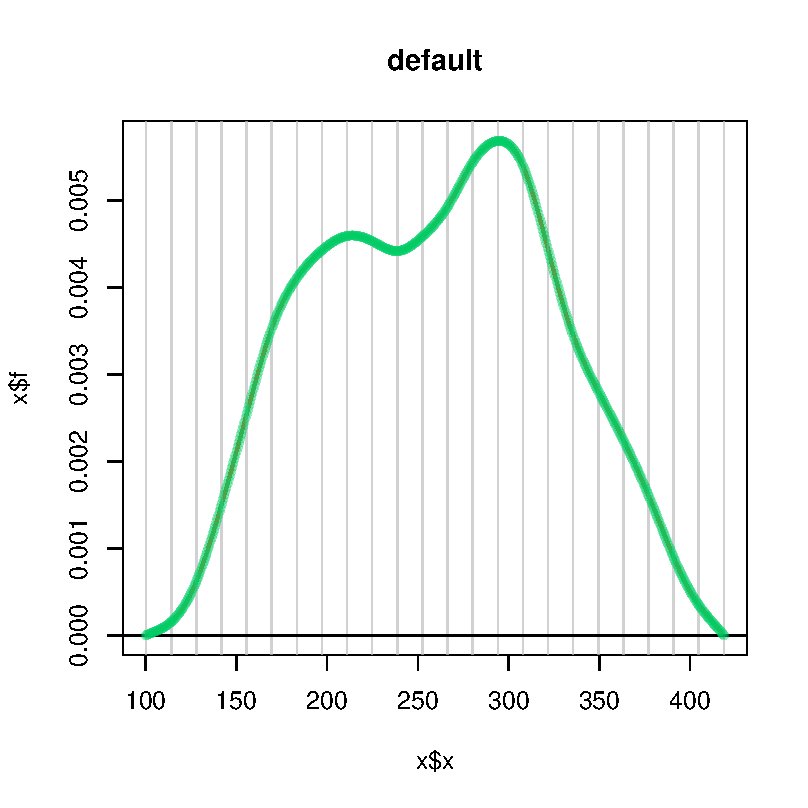
\includegraphics[width=7.4cm]{Rgraphics/figSplineDens1-1.pdf} &
     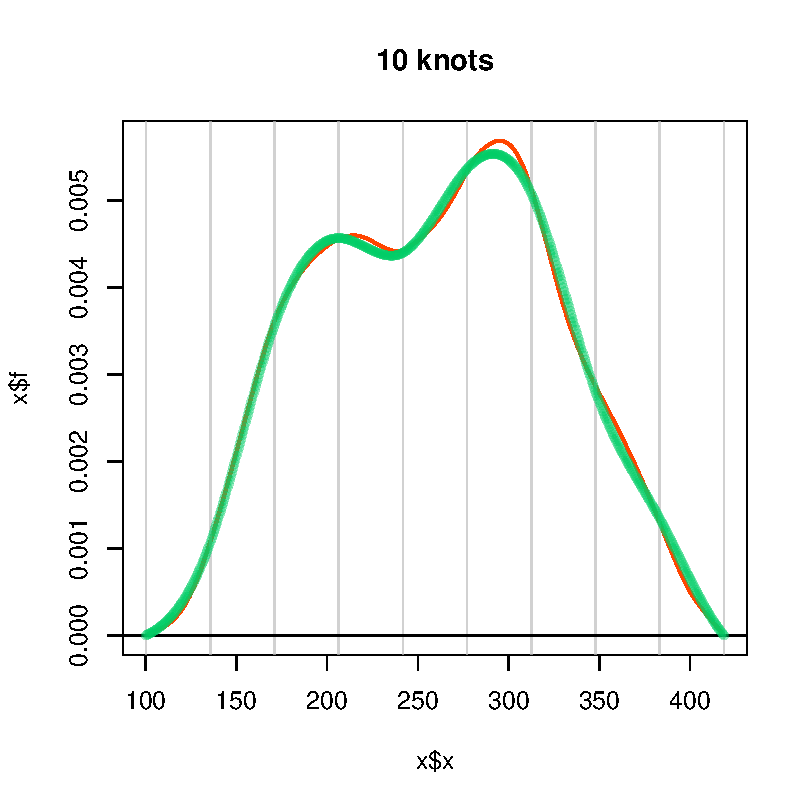
\includegraphics[width=7.4cm]{Rgraphics/figSplineDens1-2.pdf} 
   \end{tabular}
   \caption{\label{FigSplineDens} Spline density approximation for
     Brest. The original grid density (with
     512 points) is shown as a red curve in both
     cases. With only the default $24$ knots (left), the spline
     approximation is very close to the original density which is then
     hidden. With as few as $10$ knots (right), the approximation is
     quite good.}
\end{figure}

\medskip 
\index{knots (spline)} 
Knots locations are chosen by default
to be equispaced. The number of knots can be fixed with \verb@nKnots@
and the knots locations can be given as well, if needed, by using the
\verb@knots@ formal argument.  As it might be guessed from the
generated message, the created spline uses the values of the
derivatives at the two-end points $\Low{x}$ and $\Up{x}$. Here they
are computed using a finite difference approximation, but they could
have been specified.  Using good boundary conditions is often an issue
in density estimation.  The derivatives of the spline at end-points
can be prescribed thanks to a multiple knots strategy,
see appendix~\ref{AnnSpline}.

Note that the spline is fitted to the provided density by using a
least-squares criterion with the constraint that the spline density
integrates to $1$ as wanted.  Further equality constraints are used
for boundary conditions if needed. However, positivity constraints are
not used for now, which is an obvious limitation. As far as tide
densities are used with a fine grid representation, positivity
constraints will nearly hold in practice. The function
\verb@SplineDensity@ may still warn about some slightly negative
spline values, with no serious consequence.

\index{warning}
\index{constraint!normalisation}
\index{constraint!positivity}

\begin{remark}
  Cubic splines with positivity constraints could be coped with using
  Second Order Constrained Programming (SOCP),~\cite{PappAlizadeh}.
\end{remark}

The S3 class \verb@"GPDtail"@ describes distributions which result
from the convolution of spline density and a GPD. The \verb@GPDtail@
function is used to create an object of this class.

\begin{knitrout}
\definecolor{shadecolor}{rgb}{0.969, 0.969, 0.969}\color{fgcolor}\begin{kframe}
\begin{alltt}
\hlkwd{set.seed}\hlstd{(}\hlnum{1234}\hlstd{)}
\hlstd{u} \hlkwb{<-} \hlnum{50}
\hlstd{par.y} \hlkwb{<-} \hlkwd{c}\hlstd{(}\hlstr{"scale"} \hlstd{=} \hlkwd{rgamma}\hlstd{(}\hlnum{1}\hlstd{,} \hlkwc{shape} \hlstd{=} \hlnum{2}\hlstd{,} \hlkwc{scale} \hlstd{=} \hlnum{30}\hlstd{),}
           \hlstr{"shape"} \hlstd{=} \hlnum{0.2} \hlopt{*} \hlkwd{runif}\hlstd{(}\hlnum{1}\hlstd{))}
\hlstd{res} \hlkwb{<-} \hlkwd{GPtail}\hlstd{(}\hlkwc{x} \hlstd{= SD,} \hlkwc{par.y} \hlstd{= par.y,} \hlkwc{threshold.y} \hlstd{= u,} \hlkwc{lambda} \hlstd{=} \hlnum{1}\hlstd{)}
\end{alltt}
\begin{verbatim}
## o Period for return levels (pred.period)
##  [1] 1e+00 2e+00 5e+00 1e+01 2e+01 3e+01 4e+01 5e+01 6e+01 7e+01 8e+01 9e+01
## [13] 1e+02 2e+02 5e+02 1e+03 1e+04 1e+05
## ymax =    Inf
## E.y =   13.2 sd.y =   14.2
## o computing the expectation of the exponential tail: muStar.x = 354.625
## o Using closed form smax =      716
\end{verbatim}
\begin{alltt}
\hlkwd{class}\hlstd{(res)}
\end{alltt}
\begin{verbatim}
## [1] "GPtail"
\end{verbatim}
\begin{alltt}
\hlkwd{plot}\hlstd{(res)}
\hlkwd{plot}\hlstd{(res,} \hlkwc{which} \hlstd{=} \hlnum{3}\hlstd{)}
\end{alltt}
\end{kframe}
\end{knitrout}

\noindent
The \verb@plot@ method for this class produces by default a plot
showing the three densities as shown on figure~\ref{SplineDens2-1}.
It has a \verb@which@ argument that can be used to produce a different
plot, the return level plot as on figure~\ref{SplineDens2-2} being
obtained with \verb@which = 3@ (this value is consistent with the
\pkg{evd} package).  
\index{plot method@{\texttt{plot} method}}


The call to \verb@GPtail@ is not unlike a call to \verb@convSL@. The 
probability distribution is not given here, because only the GPD can 
be used. Note that the name \verb@"GPtail"@ can be misleading because
the distribution of $Z$ resulting from the convolution does not have a GPD
tail but is tail-equivalent to a GPD for $\xi_Y>0$.
\index{tail-equivalent}

\begin{figure}
   \centering
   \begin{tabular}{c} 
     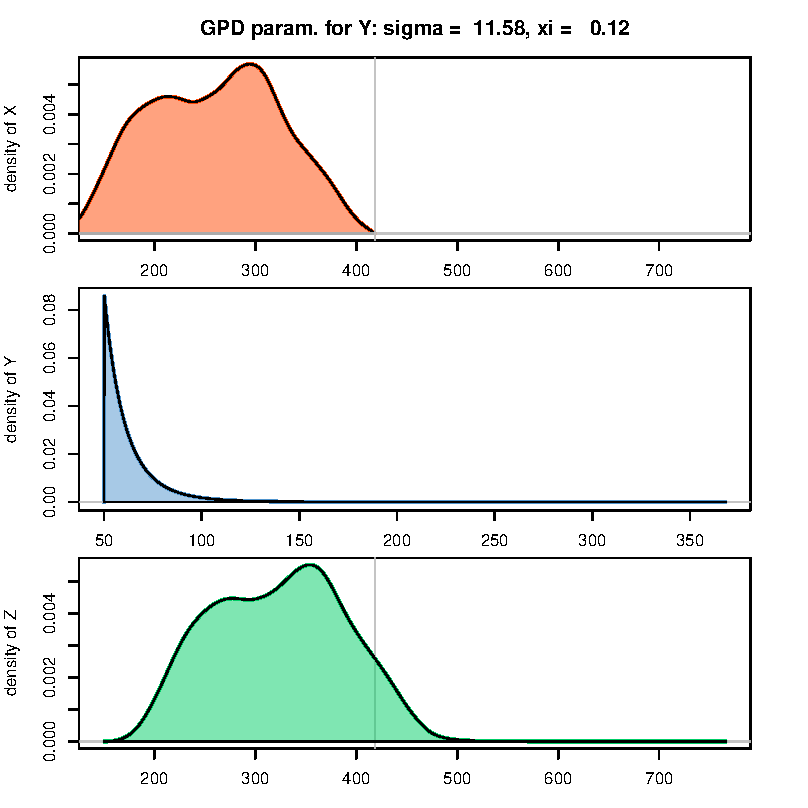
\includegraphics[width=12cm]{Rgraphics/figSplineDens2-1.pdf}
   \end{tabular}
   \caption{\label{SplineDens2-1} Convolution of a spline density and
     a GPD. The density of $Z$ seems similar to that of
     $X$ with a shift, but $Z$ has heavy tail, and is tail-equivalent to $Y$.  }
\end{figure}

\begin{figure}
   \centering
   \begin{tabular}{c c} 
     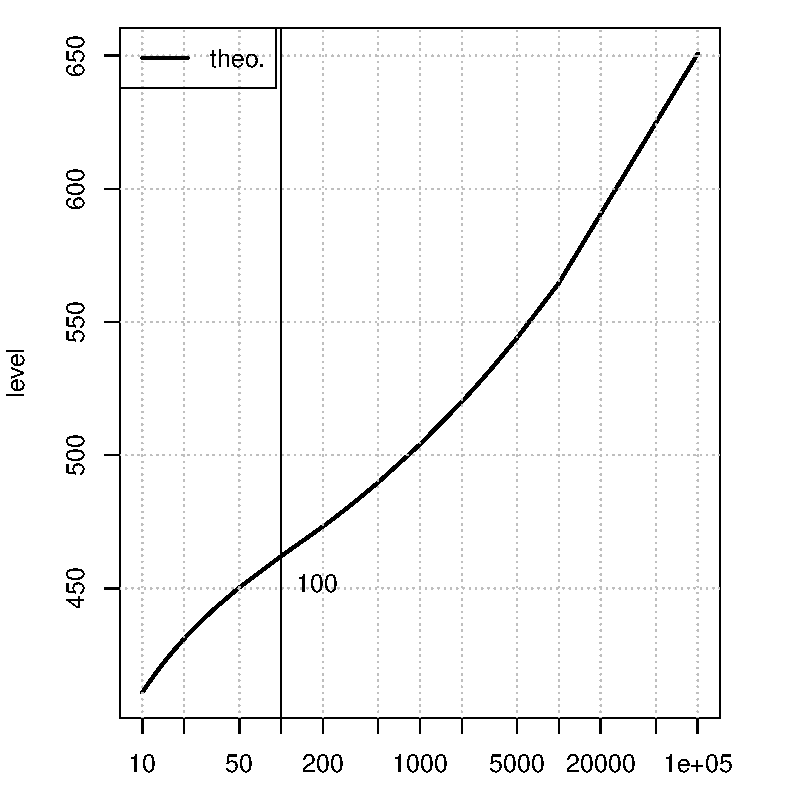
\includegraphics[width=7.4cm]{Rgraphics/figSplineDens2-2.pdf}
     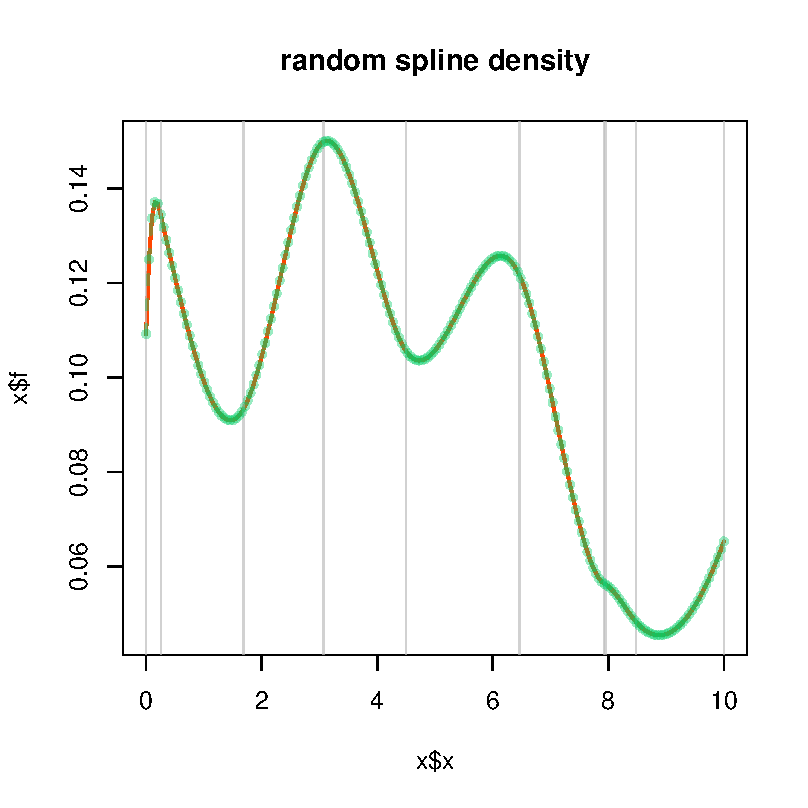
\includegraphics[width=7.4cm]{Rgraphics/figSplineDens3-1.pdf}
   \end{tabular}
   \caption{\label{SplineDens2-2} Left: Return level for the
     convolution of a spline density and a GPD for Brest data. Right:
     a random spline density.  }
\end{figure}



\section{Using \texttt{"SplineDensity"} objects}
%%-------------------------------

\subsection{Evaluation}
%%----------------------------------------------------
\index{predict method@{\texttt{predict} method}} The \verb@predict@
method can be used to evaluate the density at some chosen points. The
result is given as a list with two elements \verb@x@ and \verb@y@ and
thus it can straightforwardly be plotted.
For example, the spline density can be evaluated on a very
fine grid if needed.

\begin{knitrout}
\definecolor{shadecolor}{rgb}{0.969, 0.969, 0.969}\color{fgcolor}\begin{kframe}
\begin{alltt}
\hlstd{pred} \hlkwb{<-} \hlkwd{predict}\hlstd{(SD,} \hlkwc{newdata} \hlstd{=} \hlkwd{seq}\hlstd{(}\hlkwc{from} \hlstd{=} \hlnum{200}\hlstd{,} \hlkwc{to} \hlstd{=} \hlnum{300}\hlstd{,} \hlkwc{by} \hlstd{=} \hlnum{0.1}\hlstd{))}
\hlkwd{names}\hlstd{(pred)}
\end{alltt}
\begin{verbatim}
## [1] "x" "y"
\end{verbatim}
\end{kframe}
\end{knitrout}

\subsection{Moments/cumulants generating function}
%%----------------------------------------------------
\index{cumulants (generating function of)}
The \verb@momGen@ function can be used to provide an accurate
evaluation of the moment generating function $M_X(t) = \Esp[\exp(tX)]$ 
or of the cumulant generating function $K_X(t) = \log M_X(t)$. The
later function is useful to assess the impact of a tide $X$
for an exponential or nearly exponential surge $Y$, see section~\ref{ExpSurges} 
above.



\subsection{Random \texttt{SplineDensity}}
%%----------------------------------------------------
With the goal of testing the computations, a \verb@rSplineDensity@
function has been written to generate a random spline density with
given support. 

\begin{knitrout}
\definecolor{shadecolor}{rgb}{0.969, 0.969, 0.969}\color{fgcolor}\begin{kframe}
\begin{alltt}
\hlkwd{set.seed}\hlstd{(}\hlnum{1234}\hlstd{)}
\hlstd{SDrand} \hlkwb{<-} \hlkwd{rSplineDensity}\hlstd{(}\hlkwc{order} \hlstd{=} \hlnum{4}\hlstd{,} \hlkwc{xmax} \hlstd{=} \hlnum{10}\hlstd{)}
\hlkwd{plot}\hlstd{(SDrand,} \hlkwc{main} \hlstd{=} \hlstr{"random spline density"}\hlstd{)}
\end{alltt}
\begin{verbatim}
## NULL
\end{verbatim}
\end{kframe}
\end{knitrout}

\begin{remark}
  The simulated density is obtained using a B-spline basis and
  positive coefficients. We know that in this way we do not obtain an
  arbitrary positive spline because a spline with some negative
  coefficients still can take be a positive function. However, the densities
  generated in this way can take fairly different shapes as needed in
  checks.
\end{remark}

\index{spline density|)}

\chapter{Frequently Asked Questions}
%%==============================================
\section{Calling \texttt{convSL}}
%%-------------------------------
\noindent
\textbf{Q.} Calling \verb@convSL@, I get an error with a message 
concerning a function \verb@qfun.y@.
\par\medskip\noindent
\textbf{A.} A plausible explanation is that the distribution for the
surge does not belong to the list of special distributions and that it
does not meet the requirements about functions names. In the second
case, it may be possible to redefine the probability functions by
using a ``wrapper''. For instance, if the distribution depends on a
parameter \verb@bar@ and has density \verb@foodens@, a new density is
defined 
\begin{knitrout}
\definecolor{shadecolor}{rgb}{0.969, 0.969, 0.969}\color{fgcolor}\begin{kframe}
\begin{alltt}
\hlstd{dMydist} \hlkwb{<-} \hlkwa{function}\hlstd{(}\hlkwc{x}\hlstd{,} \hlkwc{bar}\hlstd{)} \hlkwd{foodens}\hlstd{(x,} \hlkwc{bar} \hlstd{= bar)}
\end{alltt}
\end{kframe}
\end{knitrout}
In order to use \verb@"Mydist"@ as a possible \verb@distname.y@ choice, 
the same thing must be done for the
distribution and the quantile functions which must have name
\verb@pMydist@ and \verb@qMydist@.

%%---------------------------------------------------------
\par\medskip\noindent
\textbf{Q.} I do not want to use a threshold $u$ for $Y$ nor to describe
excesses, but rather to use a known distribution for~$Y$.
\par\medskip\noindent
\textbf{A.}
Make sure that the distribution meet the requirements on probability 
functions (see question above), and proceed as in the example
of \ref{NONPOT} page~\pageref{NONPOT}.
% This situation morally corresponds to $u=-\infty$. However $Y-u$ is
% then meaningless.  A possible solution is to take a very small value
% for $u$ (say $u=-100$ if $Y$ is in meters) and to unshift the
% distribution of $Y$ using the \verb@shift.y@
%%--------------------------------------------------------
\par\medskip\noindent
\textbf{Q.} I have a warning message when calling \verb@convSL@ mentioning that
something \texttt{"is not a graphical parameter"}.
\par\medskip\noindent
\textbf{A.}  Due to the \verb@dots@ mechanism, no check is possible
for the formal arguments of \verb@convSL@. When a formal argument is not
found in the list of arguments for \verb@convSL@ it is passed to
\verb@RSLplot@ and possibly then to \verb@plot@.  When a formal is
given which does not belong to any of the three argument lists, a
message is addressed containing the above mentioned words. The formal will not be taken
into consideration Most likely, it is a misuse, and \textbf{the message 
must be read carefully}.



\section{Inference}
%%-------------------------------
\noindent
\textbf{Q.} The confidence intervals for return levels are of decreasing width 
when the level $z$ increases, which seems unnatural.
\par\medskip\noindent
\textbf{A.} Such a phenomenon can occur when the uncertainty about parameters is dominated
by the uncertainty on the rate $\lambda$. In the estimation variance of a return
level~$z(T)$, the part that can be attributed to $\lambda$ is computed using the
second partial derivative of (\ref{eq:DERT}) for  $\lambda =\widehat{\lambda}$. This gives
$$
    \Var( \widehat{\lambda} ) \times [ \partial z /\partial \lambda ]^2  =
   \Var( \widehat{\lambda} ) \times \widehat{\lambda}^{-4} T^{-2} f_Z(z)^{-2} 
$$
It might be the case that $T^{-2} f_Z(z)^{-2}$ is decreasing with~$T$. 
Note however that the uncertainty on the parameters of $Y$ is
usually the main source of uncertainty on the return levels for large
periods. Decreasing widths for the confidence intervals can also
result from a misuse of a fitted model: wrong units, error in
parameter names or order, etc.
%%--------------------------------------------------------
\section{Numerical precision}
%%-------------------------------
\noindent
\textbf{Q.} What about the numerical error? What is the maximal period
that can be trustfully be used?
\par\medskip\noindent
\textbf{A.} The numerical precision depends on the distributions used for $X$
and $Y$, and no general indication can be given. As an order of magnitude, the
use of probability of exceedances about $10^{-6}$ or even $10^{-7}$ seems viable
in \verb@convSL@ for distributions of surges with a tail close to the
exponential, as met in practice. The largest return levels will then be evaluated with a precision
close to $1\%$. With the \verb@GPtail@ function, the precision should be better,
but this still needs more investigations.


\appendix

\chapter{Numerical computation}
%%----------------------------------
\section{Discrete  convolution}
%%--------------------------------
In this section we will consider vectors with $0$ as starting index,
e.g. a vector $\m{a}$ of length $N$ writes 
$$
   \m{a} = [ a_0,\,a_1,\,\dots,\,a_{N-1}]^\top
$$
Such a vector can be related to the polynomial
$$
  a(\lambda) = a_0 + a_1\,\lambda + a_1\,\lambda^2 + \dots 
  + a_{N-1} \,\lambda^{N-1}
$$
Using two vectors $\m{a}$ and $\m{b}$ of length $N$ we can
compute their convolution product which is the vector~$\m{c}=[c_n]_n$
\begin{equation}
  \label{eq:CONV}
  c_n  = \sum_{k=0}^n a_{k}\,b_{n-k} 
  = \sum_{k,\,\ell \geqslant 0, \:k+\ell=n} a_{k}\,b_{\ell} 
\end{equation}
Note that $c_n$ is coefficient of $\lambda^n$ in the product of the two polynomials
related to $\m{a}$ and $\m{b}$ i.e.  $c(\lambda)= a(\lambda)\,b(\lambda)$. On a
plane grid of points with integer coordinates $(k,\,\ell)$, the coefficient is
obtained by summing products $a_kb_\ell$ on the line with equation $k+\ell =n$
with slope $-1$ (see figure \ref{FIGCONV}).

The product $c_n$ can be computed for any index $n\geqslant 0$ using the convention
that $\m{a}$ and  $\m{b}$ are completed by zeros e.g. $a_k=0$ for $k \geqslant N$.
Then $c_n$ can differ from zero for $n$ between $0$ and $2N-2$. Taking
$n=2N-2$ the sum (\ref{eq:CONV}) reduces to one summand
for $k=N-1$, namely $a_{N-1}\,b_{N-1}$ (see figure \ref{FIGCONV}). In other words
the convolution of two vectors of length $N$ has length $2N-1$.

It can be remarked that 
$$
    \sum_{n} c_n = \left[\sum_{k} a_k \right]
    \left[\sum_{\ell} b_\ell \right]
$$
which is easily checked using  $c(\lambda) = a(\lambda)b(\lambda)$ for $\lambda=1$.

\begin{figure}
   \centering
   \begin{tabular}{c c} 
     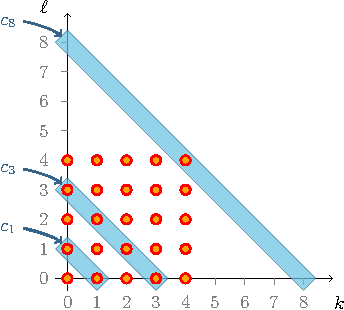
\includegraphics[width=5cm]{images/Convol.pdf} &
     %%\includegraphics[width=7.4cm]{Rgraphics/figRenplotGaronne.pdf} 
   \end{tabular}
   \caption{\label{FIGCONV} Convolution of two vectors of length $N=5$.
    If each point $[k,\,\ell]$ shows the product  $a_k\,b_\ell$, 
    then $c_n$ comes by summation over a segment of the line $k+\ell =n$. 
    For $n=2N-2$ (here $n=8$), the sum boils down to $k=\ell=N-1$.}
\end{figure}

\section{Continuous convolution}
%%---------------------------------
\subsection{Grids}
%-----------------
\index{convolution!discrete}
Consider the convolution integral of~(\ref{eq:CONVDENS})
\begin{equation}
   \label{eq:CONVDENS2}
   f_Z(z)
   = \int_{x_{\textrm{min}}}^{x_{\textrm{max}}} f_X(x)\,f_Y(z-x)\,\textrm{d} x
\end{equation}
The densities $f_X(x)$ and $f_Y(y)$ will be used in relation with 
two discrete regular grids $x_k$ and $y_k$. The two grids are assumed 
to have the same step~$h$ and the same number $N$ of intervals. For the $x$-grid, 
the intervals are $(x_k,\,x_{k+1})$ with
$$
    x_0 < x_1 < \dots < x_{N}  \qquad x_k = x_0 + k\times h \quad  (k \textsf{ integer})
$$
and similarly let $y_\ell= y_0+\ell \times h$ for integer~$\ell$. The grid
$x_k$ is assumed to cover the support of $f_X(x)$, i.e. $x_0 \leqslant
x_{\textrm{min}}$ and $x_{\textrm{max}} \leqslant x_N$.  Then from (\ref{eq:CONVDENS2})
\begin{equation}
  \label{eq:CONV0N}
  f_Z(z)
   = \int_{x_{\textrm{min}}}^{x_{\textrm{max}}} 
   = \int_{x_{0}}^{x_{N}} = \sum_{k=0}^{N-1} \int_{x_{k}}^{x_{k+1}}
\end{equation}
where all integrals share the same integrand as (\ref{eq:CONVDENS2}). Consider
the sequence $a_k$ and $b_k$ formed by the values of the densities $f_X(x)$ and
$f_Y(y)$ at grid points
\begin{equation}
  \label{eq:ABRECT}
    a_k = f_X(x_k), \quad b_k = f_Y(y_k) \qquad 0 \leqslant k \leqslant N-1
\end{equation}
with the convention $a_k$ and $b_k$ are zero when $k<0$ or $k>N-1$.  
Let $z_0 = x_0 + y_0$ and $z_n = z_0 +n \times h$ for integer $n$. Then $z_n
-x_k=y_{n-k}$ for all $n$, $k$.

\subsection{Rectangles or trapezes}
%-----------------------
The rectangles approximation for~$f_Z(z)$ replaces each integral
$\int_{x_{k}}^{x_{k+1}}$ in~(\ref{eq:CONV0N}) by the product of the length $h =
x_{k+1} - x_k$ and the integrand at~$x_k$. This gives
\begin{equation}
  \label{eq:RECT}
   \int_{x_{k}}^{x_{k+1}}f_X(x)\,f_Y(z-x)\,\mathrm{d}x 
   \approx  h f_X(x_k)f_Y(z - x_k) 
\end{equation}
Replacing $z$ by $z_n$ and summing for $k=0$ to $k=N-1$, we get
\begin{equation*}
   \label{eq:APPROX}
  f_Z(z_n) \approx h \,\sum_{k=0}^{N-1} a_k b_{n-k}
  %% = h \, c_n
\end{equation*}
The sum at right hand side has the same summand as the 
convolution product $c_n$, but the sum runs from $k=0$ to $n$ for $c_n$, against
$k=0$ to $N-1$ here. The two sums are identical for $0 \leqslant n \leqslant 2N-1$, i.e.
\begin{equation}
  \label{eq:IDENT}
  \sum_{k=0}^{N-1} a_k b_{n-k} = \sum_{k=0}^{n} a_k b_{n-k} \qquad \textrm{for}\quad 
  0 \leqslant n \leqslant 2N-1
\end{equation}
The reason is that $a_k$ and $b_{\ell}$ are zero when $[k,\,\ell]$ is outside
the square $0 \leqslant k,\,\ell \leqslant N-1$ (see figure~\ref{FIGCONV}).  
Note however that $f_Y(y_\ell)$ is only \textit{approximately zero} and
that the square side $Nh$ must be chosen with care, see~\ref{CHOOSEGRID}.

The rectangles rule is known to be less precise than the trapezoidal rule which
has the same computational cost, and the later is always preferred. The integral
$\int_{x_{k}}^{x_{k+1}}$ in~(\ref{eq:CONV0N}) is then approximated by the
product of the length $h$ and the mean value of the integrand at the two
end-points~$x_k$ and $x_{k+1}$
\begin{equation}
  \label{eq:TRAP}
  \int_{x_{k}}^{x_{k+1}}f_X(x)\,f_Y(z-x)\,\mathrm{d}x 
  \approx \frac{h}{2} \left\{ f_X(x_k)f_Y(z - x_k) + f_X(x_{k+1})f_Y(z - x_{k+1}) \right\}
\end{equation}
%% Replacing $z$ by $z_n$, summing for $k=0$ to $k=N-1$ and using simple 
%% algebra we get
%% \begin{equation}
%%   \label{eq:TRAPFORM}
%%    f_Z(z_n) \approx \frac{1}{2h} \left\{ 2 \sum_{k=0}^{N-1} a_k b_{n-k} 
%%      - a_0 b_n + a_N b_{n-N}\right\}
%% \end{equation}
%% for $0 \leqslant n \leqslant N-1$. 
When $a_0=0$ and $a_N=0$, the trapezoidal rule leads unsurprisingly
to the same computation as the rectangles rule.

%%\subsubsection{Modified trapezoidal}
%%-----------------------------
%% Rather than $b_k=f_Y(y_k)$, we can consider the mean value $b_k^\star$ of $f_Y(y)$ on the
%% interval~$(y_{k-1},\,y_{k})$
%% \begin{equation}
%%   \label{eq:AK}
%%   b_k^\star = \frac{1}{h}\,\int_{y_{k-1}}^{y_{k}} f_Y(y)\,\textrm{d}y = 
%%     \frac{1}{h}\,\left\{ S_Y(y_{k-1}) - S_Y(y_k) \right\}
%% \end{equation}
%% for $0 \leqslant k \leqslant N-1$, with the convention $S_Y(y_{k})=1$
%% for $k = -1$.  This choice uses the fact that $S_Y(y)$ is available
%% for exact computation, and ensures that the vector
%% $\m{b}^\star$ has unit sum. The mean value theorem tells that
%% $$
%%   \int_{x_{k}}^{x_{k+1}} f_X(x)\,f_Y(z_n-x)\,\mathsf{d}x 
%%   = f_X(\zeta_{n,k}) \times \int_{x_{k}}^{x_{k+1}} f_Y(z_n-x)\,\mathsf{d}x 
%% $$
%% for some $\zeta_{n,k}$ between $x_k$ and $x_{k+1}$. Actually, $f_X(x)$
%% is continuous and $f_Y(z-x)$ does not change of sign on the
%% interval. Thus
%% $$
%% \int_{x_{k}}^{x_{k+1}} f_X(x)\,f_Y(z_n-x)\,\mathsf{d}x =
%% f_X(\zeta_{n,k}) \times \int_{z_n-x_{k+1}}^{z_n-x_{k}}
%% f_Y(y)\,\mathsf{d}y = h \,f_X(\zeta_{n,k}) \,b_{n-k}^\star
%% $$
%% A reasonable approximation for the unknown $f_X(\zeta_{n,k})$ is the average
%% of the values of $f_X(x)$ at the two end-points $x_k$ and $x_{k+1}$.
%% This suggests the use of the following vectors 
%% \begin{equation}
%%   \label{eq:ABRECT2}
%%    a_k^\star = \frac{1}{2} \left\{f_X(x_k) + f_X(x_{k+1}) \right\}, \quad
%%    b_k^\star =  
%%     \frac{1}{h}\,\left\{ S_Y(y_{k-1}) - S_Y(y_k) \right\} \qquad 0 \leqslant k \leqslant N-1
%% \end{equation}
%% Then the approximation of the values $f_Z(z_n)$ is obtained by
%% discrete convolution as in the rectangular case, but using
%% $\m{a}^\star$ and $\m{b}^\star$ in place of $\m{a}$ and $\m{b}$.

%% Using some simple algebra, it can be shown that for $0\leqslant n \leqslant N-1$
%% \begin{equation}
%%   \label{eq:TRAPMFORM}
%%   \sum_{k=1}^{N-1} a_k^\star \,b_{n-k}^\star 
%%      = \frac{1}{2h} \,\left\{ 
%%        + \sum_{k=0}^{N-1} a_k \left[ B_{n-k-1} -B_{n-k+1} \right]
%%         -a_0 \left[ B_n-B_{n+1} \right]
%%        +a_N \left[ B_{n-N}-B_{n+1-N} \right] 
%%        \right\}
%% \end{equation}
%% where $B_k=S_Y(y_k)$ for $0\leqslant k \leqslant N-1$ (the sequence $B_k$ is
%% decreasing).  When the density $f_X(x)$ vanishes at its end-points, we have
%% $a_0=a_N=0$ and the convolution of $\m{a}^\star$ and $\m{b}^\star$ can be
%% computed as that of $\m{a}$ and $\m{b}^\dag$ with
%% \begin{equation}
%%   \label{eq:BDAG}
%%   b_k^\dag = \frac{1}{2h} \left\{S_Y(y_{k-1})- S_Y(y_{k+1})\right\} 
%%   \qquad 0 \leqslant k \leqslant N-1
%% \end{equation}
%% which is a centred difference approximation of $f_Y(y_k)$.  Note that the right
%% hand of the formula~(\ref{eq:TRAPMFORM}) is similar to that
%% of~(\ref{eq:TRAPFORM}), but each $b_k$ is replaced by a difference
%% approximation.




\subsection{Moderate return levels: discrete convolution}
%%------------------------------
\label{CHOOSEGRID}
While the support of $X$ is assumed to have finite bounds $\Low{x}$
and $\Up{x}$, the support of $Y$ will in most cases be infinite with
$\Up{y} = +\infty$. Then we need to fix a suitable finite upper limit
$\Up{y}^\star$ in the computations.  Inasmuch as the density $f_Y(y)$
can be infinite at $\Low{y}$ for some distributions of
interest\footnote{Such as Weibull or gamma distributions with
  decreasing hazards.}, we will replace the lower end-point $\Low{y}$
by $\Low{y^\star}$ with $S_Y(\Low{y^\star}) = 1 - \varepsilon$ and
$\varepsilon>0$ is chosen small.  Then the value of $f_Z(z)$ and
$F_Z(z)$ will be computed by discrete convolution for $y$ in the
interval $(\Low{y^\star}, \,\Up{y^\star})$ where $\Up{y^\star}
\leqslant \Up{y}$ is chosen with the constraint that the computing
range $\Up{y^\star} - \Low{y^\star}$ is not too large compared to
$\Up{x} - \Low{x}$. So the density of $Z$ computed in this way will be
only for values $z \leqslant \Up{x} + \Up{y^\star}$.
\index{convolution!algorithm}

%% The discrete convolution part proceeds as follows. The technical
%% parameters to be chosen are: $N$, the chosen grid length, and $k$
%% which should be between $1$ to $4$ for the sake of numerical
%% precision.

%% \begin{enumerate}
%%   \item Let $H = \Up{x} - \Low{x}$. 
%%   \item Compute $\Low{y^\star} =q_Y(\Low{\varepsilon})$,
%%     and $\Up{y^\star} := \Low{y^\star} + k H_X$.
%%   \item Fix the grid step $h$ using $h = H/N$.
%%   \item Let $x_0 = \Low{x}$, $y_0 =  \Low{y^\star}$ and $z_0 = x_0 + y_0$.
%%   \item Fill the two vectors $\m{a}$ and $\m{b}$ of length $N$ with
%%     elements~(\ref{eq:ABRECT}), using linear interpolation for $\m{a}$.  
%%   \item Compute the convolution product vector $\m{c}$.
%% \end{enumerate}

The discrete convolution can rely on the \verb@convolve@ functionfrom
the \code{stats} package. This function uses the Fast Fourier
Transform (FFT) hence is very fast.

\begin{remarks} 
  
\item The previous algorithm only describes the computation of
  $f_Z(z)$ at grid values~$z_n$. Several results are obtained using a
  similar convolution: approximated confidence limits (delta method),
  conditional expectation $\Esp\bCond{X}{Z=z}$. See the code of the
  function \verb@convSL@ for more details.
  
\item In the cases where the surge distribution has unbounded density
  either at $\Low{y}$ or at $\Up{y}$, the results must be considered
  with care. A GPD density is always finite at $\Low{y}$; it infinite
  at $\Up{y}$ when $\xi < -1$ which is unlikely to occur in practical
  situations.
  
\end{remarks}


\subsection{Large return periods: quadratures}
%----------------------------------------------------------
The discrete convolution works fine as far as the used range of $Y$
remains comparable to the range of $X$, for instance the discretised
range $\Up{y^\star} -\Low{y^\star}$ remains $\leqslant 3 \left[\Up{x}
  -\Low{x}\right]$.  But if the upper end-point of $Y$ is $\infty$ and
if very large return periods are needed, e.g. for $T > 10^4$~years,
the discrete convolution might not be accurate enough. The reason is
that the discrete grids for $X$ and $Y$ must have the same
step~$h$. But if $\Up{y^\star} -\Low{y^\star}$ is very large, then
either the chosen step $h$ will be too large to provide a good
description of the density of $X$, or the number $N$ of grid points
will be very large. Though a large value of $N$ has a limited impact
on the computation time, it still has a nasty effect on the accuracy
of the results.

Fortunately enough, the function $S_Z(z)$ will in practice have only
quite slow variations for large $z$. So the survival $S_Z(z)$ can be evaluated
at some sparse large values rather than on a fine grid of large values. No more than 
two dozens of points are needed  for, say,  $10^3 \leqslant T \leqslant 10^7$. For one given
value of $z$, the value of the density $f_Z(z)$ as given by formula~(\ref{eq:CONVDENS2})
can be evaluated accurately by using a quadrature with a few hundreds 
of points. So a discrete convolution can be used for moderately large periods,
while a few quadratures can be used for larger periods, see figure~\ref{FigQuadPoints}.

\begin{figure}
   \centering
   \begin{tabular}{c c} 
     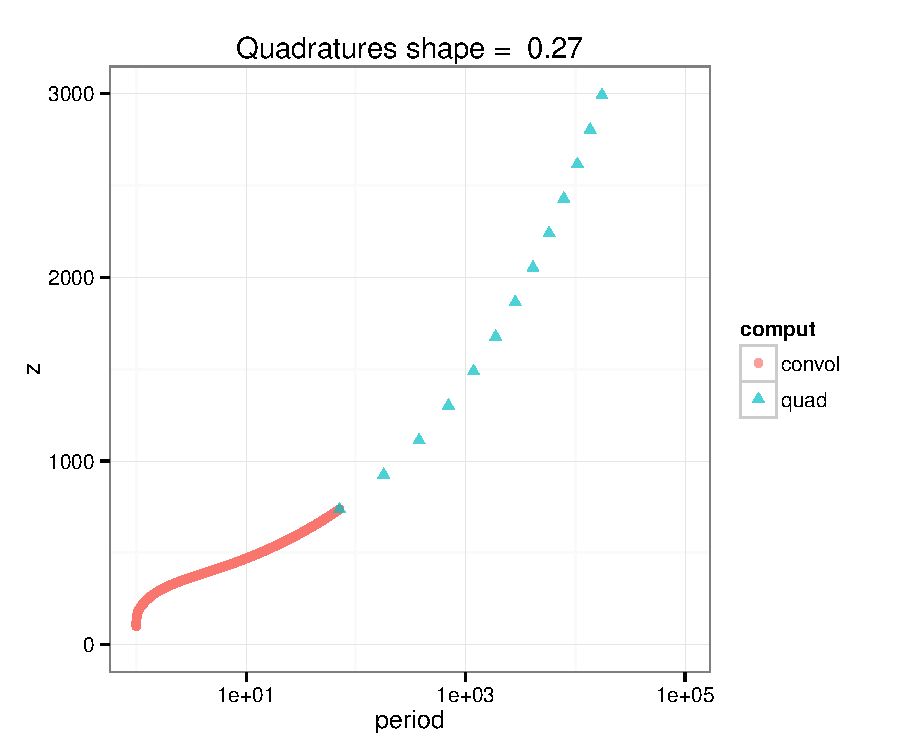
\includegraphics[width=10cm]{images/QuadPoints.pdf} &
     %%\includegraphics[width=7.4cm]{Rgraphics/figRenplotGaronne.pdf} 
   \end{tabular}
   \caption{\label{FigQuadPoints} A discrete convolution can be used
     to compute the return levels for moderately large periods. A few
     quadratures can then be used for larger periods. Note that the
     two parts of the curve are smoothly connected.}
\end{figure}

\section{Spline tide density and GPD surges}
%%---------------------------------------------------------
\label{AnnSpline}
\index{spline density|(}
\subsection{Knots}
%%---------------
\index{knots (spline)}
In this section,  the density $f_X(x)$ will be assumed to be a spline
of order~$k \geqslant 1$ with a sequence~$\zeta_k$ of $\ell + 1$ knots
$$
   \zeta_0 < \zeta_1 < \dots < \zeta_{\ell}
$$
$\zeta_0 = \Low{x}$ and $\zeta_\ell = \Up{x}$. In an usual framework
this means that $f_X(x)$ coincides with a polynomial of degree
$\leqslant k-1$ on each of the $\ell$ intervals
$(\zeta_i,\,\zeta_{i+1})$ and satisfies the following $m-1$ continuity
conditions at each interior knot~$\zeta_i$ for $2 \leqslant i
\leqslant \ell -1$
\begin{equation}
  \label{eq:CONT}
  f_X^{[j]}(\zeta_i-) = f_X^{[j]}(\zeta_i+)  \qquad 
  (0 \leqslant j < k-1). 
\end{equation}
Thus if $k=2$ we impose one continuity condition at each knot, while
the cubic spline ($k = 4$) requires the continuity of the derivatives
up to the second order. A spline of order $k=1$ is simply a piecewise
constant function with no conditions.

For the two boundary knots $\zeta_0$ and and $\zeta_\ell$, the
conditions (\ref{eq:CONT}) are too strong for practical uses, because
in practice the density does not even need to be continuous there.  The
classical solution is to think of these boundary knots $\zeta_i$ as
\textit{multiple knots} with multiplicity $\nu_i$. Then the $k-\nu_i$ following
continuity conditions must hold for knot $\zeta_i$
\begin{equation}
  \label{eq:CONT2}
  f_X^{[j]}(\zeta_i-) = f_X^{[j]}(\zeta_i+)  \qquad 
  (0 \leqslant j < k - \nu_i). 
\end{equation}
So if $\nu_i=k$ the density can be discontinuous at $\zeta_i$.  At no
cost in the discussion, we can assume that each of the $\ell + 1$
knots $\zeta_i$ is multiple with multiplicity $\nu_i \geqslant 1$ and
continuity conditions (\ref{eq:CONT2}). Thus
$$
   \underset{\textrm{number of continuity conditions}}{(k - \nu_i )} 
   + \underset{\textrm{multiplicity}}{\nu_i}   = 
   \underset{\textrm{spline order}}{k}
$$
see the book by Carl de Boor~\cite{deBoor}. In the function \verb@SplineDensity@, only the two
end-knots are for now allowed to be multiple, but densities with a
discontinuous derivative at an interior knot could be considered as
well in the future. 

\subsection{B-spline Basis}
%%------------------------------
A spline density in \pkg{SeaLev} is coped with by using the B-spline
basis related to the knots sequence. The spline density writes as  
\begin{equation}
  \label{eq:BsplineDens}
  f_X(x) = \sum_i \alpha_i B_i(x)
\end{equation}
where each $B_i(x)$ is a basis B-spline with support
$(\zeta_i,\,\zeta_{i+k})$, see figure~\ref{FigBspline}.  The basis is
provided by the \verb@splineDesign@ function of the \pkg{splines} base
package~\cite{RMANUAL}. The unknown spline coefficients $\alpha_i$ 
of~(\ref{eq:BsplineDens}) are
obtained by constrained least squares. Given a grid density, its spline
approximation is found by solving a quadratic programming problem
thanks to the \pkg{quadprog} package~\cite{PACKquadprog}. The spline
coefficients $\alpha_i$ are chosen in order to minimise the sum of squares of the
differences between the grid and the spline densities at grid
points. The constraints are equality constraints: one is for the
normalisation of the density. Boundary conditions also translate
into equality constraints. The normalising constraint is
coped with by integrating the basis functions thanks to a recurrence
relation, see~\cite[p.~128]{deBoor}.
Of course, this method requires that a fine
grid is used for the provided density.



\begin{figure}
  \centering
  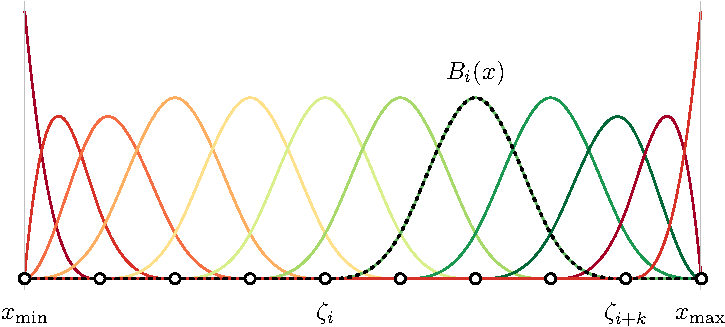
\includegraphics[width=12cm]{./figures/figure/Bspline.pdf}
  \caption{\label{FigBspline} B-spline basis functions for the
    $10$-knots example, object \texttt{SD10}, which was shown on the
    right of figure~\ref{FigSplineDens}. The locations of the knots
    $\zeta_i$ are shown by circles, with $\zeta_0 = \Low{x}$ and $\zeta_9 =
    \Up{x}$. The order is $k = 4$ (for a cubic spline). The support of
    a basis spline $B_i$ is the interval $(\zeta_i,\,\zeta_{i+k})$.  }
\end{figure}


\index{constraint!equality}
\index{constraint!normalisation}
\index{grid density}

\subsection{Some theoretical facts}
%%---------------
The following results\footnote{Which, to our best knowledge, seem new.}
are used in the \verb@momGen@ and \verb@GPtail@ functions.

\begin{theo}
  \label{lemma:LemmaMomGen}
  Assume that the density $f_X$ has support
  $[\zeta_0,\,\zeta_{\ell}]$ and has a sequence of $\ell+1$ knots
  $\zeta_i$ with multiplicities $\nu_i \geqslant 1$. 
  
  \begin{list}{$\bullet$}{ }
  \item Then the moment
    generating function of~$X$, i.e.  $M_X(t):= \Esp[e^{tX}]$ is given for $t \neq 0$ 
    by
    $$
    M_X(t) = \sum_{i=0}^\ell \, \left\{ \sum_{j = k-\nu_i}^{k-1}
      \frac{(-1)^{j+1}}{t^{j+1}} \left[ f^{[j]}_X(\zeta_i+) -
        f^{[j]}_X(\zeta_i-) \right] \right\} \, e^{t \zeta_i}.
    $$
  \item If $Y \sim \mathtt{GPD}(\mu_Y,\,\sigma_Y,\,\xi_Y)$, and 
    $1/\xi_Y$ is not equal to any of the integers $1$, $2$, $\dots$, $k$ then
    the survival function of $Z$ is given by
    \begin{equation}
      \label{eq:SSplineGPD}
      S_Z(z) = \sum_{i=0}^{\ell} \, \sum_{j=k-\nu_i}^{k-1} a_j d_i^{[j]} 
      \left[1 + \xi_Y \frac{z-\zeta_i}{\sigma_Y} \right]^{-1/\xi_Y + j +1 }   
    \end{equation}
    for all real $z > \zeta_{\ell}$, where the coefficients $d_i^{[j]}$
    are given by 
    $$
    d_i^{[j]} := 
    \left[f^{[j]}_X(\zeta_i+) - f^{[j]}_X(\zeta_i-) \right]
    $$
    for $k - \nu_i \leqslant j \leqslant k-1$, and by $d_i^{[j]} :=0$
    otherwise, while $a_j$ is given by 
  $$
  a_j := \frac{(-\sigma_Y)^{j+1}}{(1-\xi_Y)\,(1 - 2 \xi_Y)\,     
    \dots 
    (1 + (j+1) \xi_Y)}
  $$ 
  for $0 \leqslant j \leqslant k-1$. 
\end{list}
  
\end{theo}

The proof of this theorem relies on recursive integrations by
parts. Note that the expression for $S_Z(z)$ can be
derived w.r.t. the parameters of the GPD, this allows the
determination of confidence intervals for the return levels based on
the delta method.  \index{delta method}

A remarkable point in the theorem is that the coefficients $a_j$ are 
not positive. If only simple knots are used, it can be shown that
$\sum_i a_i \zeta_i^j = 0$ for $0 \leqslant j \leqslant k-1$ hence
the coefficients $a_j$ sum to zero.

\subsection{Practical consequences}
%%---------------------------------------
The formulas and the extension of the theorem above are used in the
\verb@GPDtail@ and \verb@momGen@ functions.

The first statement of the theorem can be used for exponential 
surges, since the cumulant generating function for the tide gives the 
shift between the sea level tail and the surge tail, see section~\ref{ExpSurges}.

The second statement of the theorem is used for the general case $\xi_Y \neq 0$. It
allows the accurate determination of the sea level tail distribution  
without using discrete convolution or quadratures. Since the formula
for $S_Z(z)$ only works for $z > \Up{x} + \mu_Y$, a discrete 
convolution must be used to compute the bulk of the distribution.




\index{bulk of a distribution}

\index{spline density|)}

\chapter{Validation and special cases}
%%----------------------------------
\section{Exponential Surges}
\label{AnnExpSurges}
\index{exponential distribution|(} When a POT model with exponential
distribution is used for the surge~$Y$, the exact (conditional)
distribution of $Z$ is known. More precisely, conditional on $Z >
x_{\mathrm{max}} + \mu_Y$ the random variable $Z$ then follows an
exponential distribution with shape $\sigma_Z=\sigma_Y$ and location
$\mu_Z = \mu_X^\star + \mu_Y$ where $\mu_X^\star$ was given
in~(\ref{eq:muXStar}) in section~\ref{ExpSurges}.

This result allows a simple check of the computation. The \verb@show.asympt@
argument of the \verb@convSL@ function allows us to add the theoretical
return level curve to the one computed by convolution. As an example, we can
use the computation for Brest. With the threshold $u=50$~cm, the surge
excesses can be considered as exponentially 
distributed with scale $\sigma_Y=10$~cm, i.e. with rate $1/10.0\,\mathrm{cm}^{-1}$.

\begin{knitrout}
\definecolor{shadecolor}{rgb}{0.969, 0.969, 0.969}\color{fgcolor}\begin{kframe}
\begin{alltt}
\hlstd{theta2.y} \hlkwb{<-} \hlkwd{c}\hlstd{(}\hlstr{"rate"} \hlstd{=} \hlnum{0.10}\hlstd{)}
\hlstd{conv.asympt} \hlkwb{<-} \hlkwd{convSL}\hlstd{(}\hlkwc{dens.x} \hlstd{= Brest.tide,}
                      \hlkwc{threshold.y} \hlstd{=} \hlnum{50}\hlstd{,}
                      \hlkwc{distname.y} \hlstd{=} \hlstr{"exponential"}\hlstd{,}
                      \hlkwc{lambda} \hlstd{= lambda,}
                      \hlkwc{par.y} \hlstd{= theta2.y,}
                      \hlkwc{show.asympt} \hlstd{=} \hlnum{TRUE}\hlstd{,}
                      \hlkwc{Tlim} \hlstd{=} \hlkwd{c}\hlstd{(}\hlnum{5}\hlstd{,} \hlnum{1000000}\hlstd{),}
                      \hlkwc{main} \hlstd{=} \hlstr{"Asymptotic curve: exponential Y"}\hlstd{)}
\end{alltt}
\end{kframe}
\end{knitrout}
It can bee seen on the left panel of figure~\ref{ASYMPT}
that the return level curve computed by convolution nearly 
coincides with the exact result.
\index{exponential distribution|)}

\section{GPD surges}
%%-----------------------
\label{GPDSurgesANN}
\index{GPD (Generalised Pareto Distribution)}
When a POT model with GPD distribution is used for the surge~$Y$,
the exact (conditional) distribution of $Z$ is no longer known,
but the asymptotic behaviour of the survival $S_Z(z)$ is known.

When $\xi_Y>0$ it can be shown that $S_Z(z)/S_Y(z)$ tends to~$1$ when $z \to
\infty$, but with a \textit{very slow} convergence. The return level curve
should broadly behave as if $Z$ was GPD with parameters $\sigma_Z = \sigma_Y$
(scale), and $\xi_Z = \xi_Y$ (shape). In view of the exponential case~$\xi_Y=0$,
the location parameter $\mu_Z$ can be chosen as $\mu^\star_X + \mu_Y$ where
$\mu_X^\star$ was defined in~(\ref{eq:muXStar}). Note that the tail 
equivalence does not imply that the difference between the return levels
$z(T)$ and $y(T)$ tends to zero nor even to a finite limit.

\begin{knitrout}
\definecolor{shadecolor}{rgb}{0.969, 0.969, 0.969}\color{fgcolor}\begin{kframe}
\begin{alltt}
\hlstd{theta3.y} \hlkwb{<-} \hlkwd{c}\hlstd{(}\hlstr{"scale"} \hlstd{=} \hlnum{10}\hlstd{,} \hlstr{"shape"} \hlstd{=} \hlnum{0.03}\hlstd{)}
\hlstd{conv.asympt} \hlkwb{<-} \hlkwd{convSL}\hlstd{(}\hlkwc{dens.x} \hlstd{= Brest.tide,}
                      \hlkwc{threshold.y} \hlstd{=} \hlnum{50}\hlstd{,}
                      \hlkwc{distname.y} \hlstd{=} \hlstr{"GPD"}\hlstd{,}
                      \hlkwc{lambda} \hlstd{= lambda,}
                      \hlkwc{par.y} \hlstd{= theta3.y,}
                      \hlkwc{show.asympt} \hlstd{=} \hlnum{TRUE}\hlstd{,}
                      \hlkwc{Tlim} \hlstd{=} \hlkwd{c}\hlstd{(}\hlnum{5}\hlstd{,} \hlnum{1000000}\hlstd{),}
                      \hlkwc{main} \hlstd{=} \hlkwd{sprintf}\hlstd{(}\hlstr{"Asymptotic curve: GPD Y with shape %4.2f"}\hlstd{,}
                          \hlstd{theta3.y[}\hlstr{"shape"}\hlstd{]))}
\end{alltt}
\end{kframe}
\end{knitrout}

\noindent
The plot is on the right panel of figure~\ref{ASYMPT}. 

\begin{figure}
  \centering
  \begin{tabular}{c c} 
    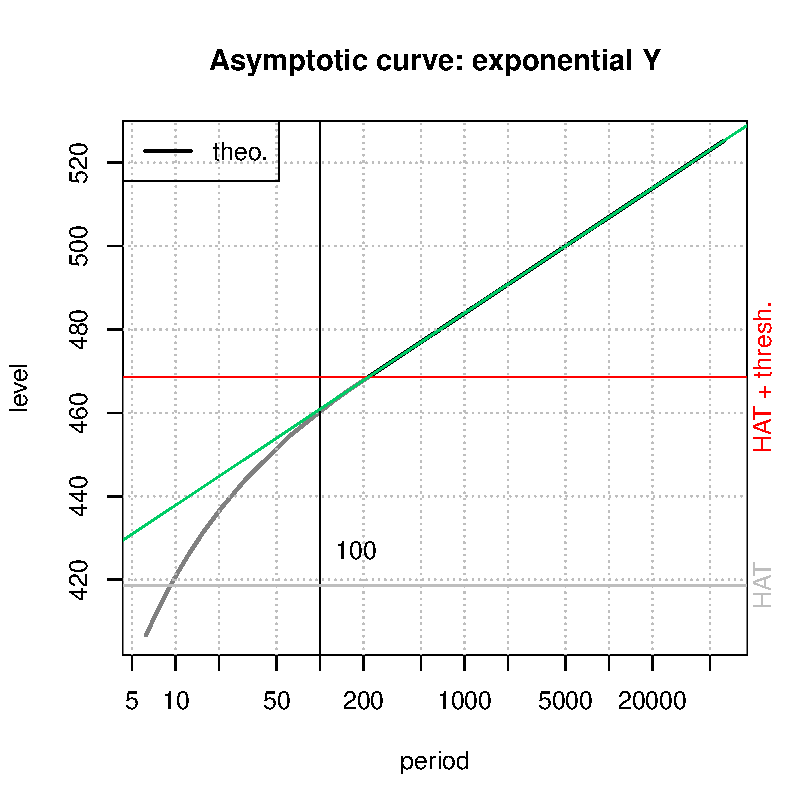
\includegraphics[width=7.4cm]{Rgraphics/figBrestAsympt1-1.pdf} &
    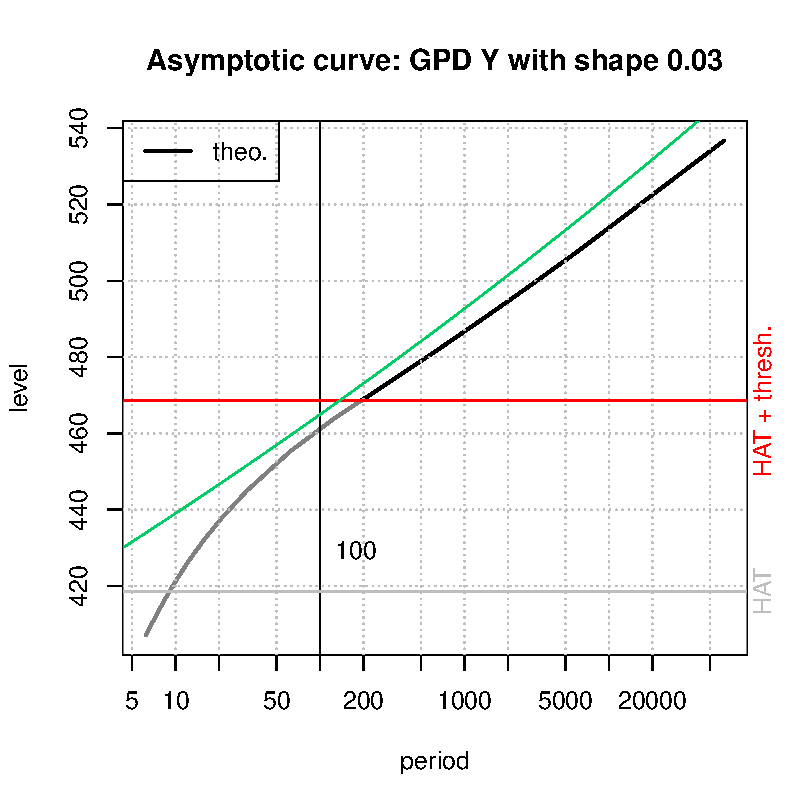
\includegraphics[width=7.4cm]{Rgraphics/figBrestAsympt2-1.pdf} 
    %% \includegraphics[width=7.4cm]{Rgraphics/figRenplotGaronne.pdf} 
  \end{tabular}
  \caption{\label{ASYMPT} Adding the asymptotic return level curve (in
    green). Left panel: exponential, right panel GPD with shape
    $\xi_Y>0$.}
\end{figure}

\section{Comparing several computations}
%%-----------------------
From \pkg{SeaLev} \verb@>= 0.4-2@ the function \verb@convSL@ function
  no longer uses a discrete convolution for the whole range of values
  of $z$. Rather, the discrete convolution is used for a limited range
  of $z$ values and quadratures are used for (sparse) large values of
  $z$. It is easily checked that the return periods computed by the
  two methods are --~as expected~-- smoothly connected at the maximal
  value $z$ for which the discrete convolution is used (sse
  figure~\ref{FigQuadPoints}). Moreover, the spline-based derivation of the tail when $Y$
  has a GP distribution provides a new validation. Indeed, the
  computations based on the closed formula are completely independent
  of those arising from quadratures. It was checked that 
  the return levels and the confidence limits are nearly identical 
  in the two cases.

\bibliography{SeaLev}
\bibliographystyle{alpha}

{%% 
  \small
  \printindex
}

\end{document}

